\chapter{Mixed FE methods with convection stabilization}
\label{chap-TBT_OSS}

\section{Introduction}
\label{sec-C5_introduction}

The VMS method for incompressible turbulent flows has been analyzed previously in Chapter \ref{chap-Rb_VMS}. As stated there, the VMS method introduced by Hughes in \cite{hughes_multiscale_1995,hughes_variational_1998} is a framework to develop stable and accurate numerical approximations of partial differential equations, preventing numerical instabilities that arise when the standard Galerkin FE method is used. 

We also recall here that the use of VMS method as an ILES method was firstly suggested in \cite{hughes_multiscale_2001,hughes_large_2001,codina_stabilized_2002} and, since then, several VMS methods have been developed and used as ILES. We can distinguish between those that introduce a three scale decomposition into resolved large and small scales and unresolved scales \cite{koobus_variational_2004,john_variants_2008, john_numerical_2010, calderer2013residual}, with a Smagorinsky type model for the influence of unresolved scales onto the small resolved ones, and those that introduce a two scale decomposition into resolved and unresolved ones \cite{bazilevs_variational_2007,colomes_assessment_2015} using a residual based or projection based model of the unresolved scales to account for their influence into the resolved ones.

In \cite{codina_stabilization_2000}, a two scale VMS approach through OSS was firstly introduced. The main idea of the OSS method is to select the space of small scales orthogonal to the FE space, in contrast to the traditional choice of taking the subscales proportional to the residual, which is called ASGS in \cite{codina_stabilization_2000}. Apart from the choice of the space of subscales, their time dependency and the VMS splitting of nonlinear terms was studied in \cite{codina_time_2007}. Several combinations of these modelling possibilities where exhaustively assessed for homogeneous and wall bounded turbulent flows in \cite{colomes_assessment_2015}\footnote{Chapter \ref{chap-Rb_VMS} collects most of the work exposed in \cite{colomes_assessment_2015}, which has been extended and adapted to fit in the argumentation of this thesis.}. In that work, an explicit algorithm to compute the orthogonal projections was used and the projection of the whole residual was considered.

An alternative definition of the OSS method was proposed in \cite{codina_analysis_2008} using a term-by-term stabilization that does not involve the full residual. A similar term-by-term stabilization approach was followed in \cite{braack_local_2006}, where the Local Projection Stabilization (LPS) method was introduced. This type of techniques are also known as symmetric projection stabilization, and the key ingredient that leads to different schemes is the definition of such projection \cite{braack_local_2006,badia_stabilized_2012}. One of the main interests of a term-by-term stabilization is that one can avoid the addition of the pressure gradient stabilization term when using \textit{inf-sup} stable (ISS) velocity-pressure pairs. Another advantage of the \textit{term-by-term} stabilization methods is that the projection can be easily treated as implicit, without having all the residual terms coupled. The use of equal-order or ISS pairs with the LPS method was assessed for laminar flows in \cite{g_lube_local_2008}, concluding that the grad-div stabilization term is more relevant than the convective stabilization term when ISS FEs are used. The same conclusion was pointed out in \cite{john_numerical_2010}, where the turbulent channel flow is studied using a projection-based and a bubble-based FE VMS method introducing a Smagorinsky type model to stabilize convection. 

The main goal of this chapter is to assess for the first time the accuracy and efficiency of convection-stabilized ISS schemes as ILES methods, where symmetric projection stabilization is used. In particular, we analyze the term-by-term OSS method with implicit treatment of the projection for turbulent flows. We also analyze the influence of the grad-div stabilization on the accuracy of the method. For ISS discretizations, the influence of this term on the mass conservation is well known \cite{linke_collision_2009} but it also influences the computational cost of the linear solvers \cite{olshanskii_grad-div_2004,heister_efficient_2013}. In this respect, we present a block preconditioning strategy that makes use of recursive block factorizations \cite{badia_block_2014} to deal with the implicit projections and with the saddle point structure of the velocity-pressure coupling, which can also be applied to equal order interpolation with pressure stabilization. The comparison of the results is made with respect to those obtained using the residual-based ASGS for which we also use a block preconditioning strategy.

This chapter is organized as follows. The Navier-Stokes equations together with some notation used in the paper are stated in Section~\ref{sec-C5_prob_statement}. The VMS framework is introduced in Section~\ref{sec-C5_VMS_framework}, which includes the final discrete formulation of the ASGS method, given in Section~\ref{subsec-C5_ASGS}, the term-by-term OSS given in Section~\ref{subsec-C5_OSStbt}, the term-by-term OSS with ISS elements given in Section~\ref{subsec-C5_OSSiss} and also a brief discussion of known properties of the grad-div stabilization given in Section~\ref{subsec-C5_pressure_subscale}. The recursive block iterative strategy proposed to solve the linear system of the monolithic problem is presented in Section~\ref{sec-C5_block_precond}. The numerical results are shown in Section~\ref{sec-C5_experiments}, where two different turbulent tests are analyzed: the Taylor-Green Vortex flow in Section \ref{subsec-C5_TGV-VMS} and the Turbulent Channel Flow in Section \ref{subsec-C5_turb_channel}. Finally, some conclusions are pointed out in Section \ref{sec-C5_conclusions}.

\section{Problem statement}
\label{sec-C5_prob_statement}
For the sake of chapter completeness, let us retrieve the problem definition described in \Chap{Preliminaries}, albeit rather briefly.

Let $\Omega$ be a bounded domain of $\mathbb{R}^d$, where $d=2,3$ is the number of space dimensions, $\Gamma=\partial\Omega$ its boundary and $(0,T]$ the time interval. The strong form of the transient Navier-Stokes problem consists in finding the velocity field $\u$ and the pressure field $p$ such that 
\begin{align}
\label{eq-C5_NS_strong_mome}
\partial_t\u-\nu\Delta\u+\u\cdot\nabla\u+\nabla p&=\f&\mbox{in $\Omega\times(0,T]$,}\\
\label{eq-C5_NS_strong_inc}
\nabla\cdot\u&=0&\mbox{in $\Omega\times(0,T]$,}
\end{align}
with $\f$ the force vector and $\nu$ the kinematic viscosity. Equations \Eq{C5_NS_strong_mome} and \Eq{C5_NS_strong_inc} need to be supplied with appropriate boundary and initial conditions. The boundary $\Gamma$ is divided into the Dirichlet ($\Gamma_D$) and the Neumann ($\Gamma_N$) parts such that $\Gamma_D\cup\Gamma_N=\Gamma$ and $\Gamma_D\cap\Gamma_N=\emptyset$. Then, the boundary and initial conditions can be written as
\begin{align}
\label{eq-C5_NS_strong_Dir}
\u&=\u_g&\mbox{on $\Gamma_D\times(0,T]$,}\\
\label{eq-C5_NS_strong_Neu}
(-p\cdot\mathbf{I}+\nu(\nabla\u+\nabla\u^T))\cdot\mathbf{n}&=\mathbf{t}_N&\mbox{on $\Gamma_N\times(0,T]$,}\\
\label{eq-C5_NS_strong_Ini}
\u(\x,0)&=\u_0(\x)&\mbox{in $\Omega\times\{0\}$,}
\end{align}
$\mathbf{n}$ being the unit outward vector normal to $\Gamma$ and $ \u_0(\x) $ satisfying $ \nabla\cdot\u_0=0 $.

From equations \Eq{C5_NS_strong_mome}-\Eq{C5_NS_strong_Ini} one can derive the weak form of the problem, which consists in finding $[\u,p]\in\mathbf{L}^2(0,T;\mathcal{V}_g)\times L^1(0,T;\mathcal{Q}_0)$ such that
\begin{equation}
\label{eq-C5_NS_weak}
(\partial_t\u,\v)+B(\u,(\u,p),(\v,q)) = \left<\f,\v\right> 
\quad\quad\forall\v\in\mathcal{V}_0,\quad\forall q\in\mathcal{Q}_0,
\end{equation}
satisfying the initial condition \Eq{C5_NS_strong_Ini} in a weak sense. Here $\mathcal{V}_0:=\mathbf{H}_0^1(\Omega)$, $\mathcal{V}_g:=\mathbf{H}_g^1(\Omega)$  and $\mathcal{Q}_0:=L^2(\Omega)/\mathbb{R}$ and the form $B(\u,(\u,p),(\v,q))$ is defined as 
\begin{equation}
\label{eq-C5_bilinear}
B(\u,(\u,p),(\v,q)):=\nu(\nabla\u,\nabla\v)+b(\u,\u,\v)-(p,\nabla\cdot\v)+(q,\nabla\cdot\u)
\end{equation}
with the trilinear form of the convective term $b(\u,\v,\w)$ defined in its skew symmetric version
\begin{equation}
\label{eq-C5_conv_skew}
b(\u,\v,\w)=\frac{1}{2}(\u\cdot\nabla\v,\w)-\frac{1}{2}(\v,\u\cdot\nabla\w)+\frac{1}{2}(\v,(\u\cdot\mathbf{n})\w)_{\Gamma_N}.
\end{equation}

\section{VMS framework}
\label{sec-C5_VMS_framework}

Let us consider a FE partition $\mathcal{T}_h$ of the domain $\Omega$ from which we can construct conforming finite dimensional spaces for the velocity $\mathcal{V}_{0,h} \subset \mathcal{V}_0$, $\mathcal{V}_{g,h} \subset \mathcal{V}_g$, and for the pressure $\mathcal{Q}_{0,h}\subset \mathcal{Q}_0$. The Galerkin FE approximation of the problem \Eq{C5_NS_weak} consists in 
finding $[\u_h,p_h]\in\mathbf{L}^2(0,T;\mathcal{V}_{g,h})\times L^1(0,T;\mathcal{Q}_{0,h})$ such that
\begin{equation}
\label{eq-C5_NS_galerkin}
(\partial_t\u_h,\v_h)+B(\u_h,(\u_h,p_h),(\v_h,q_h)) =\left<\f,\v_h\right>
\quad\quad\forall\v_h\in\mathcal{V}_{0,h},\forall q_h\in\mathcal{Q}_{0,h}.
\end{equation}
In order to overcome the numerical instabilities and, eventually, to bypass the \textit{inf-sup} condition that arises when problem \Eq{C5_NS_galerkin} is solved, we use the VMS approach \cite{hughes_multiscale_1995,hughes_variational_1998} which consists in a two-scale decomposition of spaces $\mathcal{V}_0$, $\mathcal{V}_g$ and $\mathcal{Q}_0$ as $\mathcal{V}_0=\mathcal{V}_{0,h}\oplus\widetilde{\mathcal{V}}_0$, $\mathcal{V}_g=\mathcal{V}_{g,h}\oplus\widetilde{\mathcal{V}}_g$ and $\mathcal{Q}=\mathcal{Q}_{0,h}\oplus\widetilde{\mathcal{Q}}_0$, where $\widetilde{\mathcal{V}}_0$, $\widetilde{\mathcal{V}}_g$ and $\widetilde{\mathcal{Q}}_0$ are infinite-dimensional spaces that complete the FE spaces in $\mathcal{V}_0$, $\mathcal{V}_g$ and $\mathcal{Q}_0$, respectively. Hereinafter the subscript $(\cdot)_h$ will denote the FE component and the tilde $\widetilde{(\cdot)}$ the subgrid component. Applying the two-scale decomposition to (\ref{eq-C5_NS_weak}) we obtain
\begin{align}
\label{eq-C5_NS_vms}
(\partial_t\u_h,\v_h)+(\partial_t\tilde{\u},\v_h)+B(\a;[\u_h,p_h],[\v_h,q_h])-\left(\tilde{\u},\nu\Delta\v_h+\a\cdot\nabla\v_h+\nabla q_h\right)_h\\\nonumber
-\left(\tilde{p},\nabla\cdot\v_h\right)_h=\left<\f,\v_h\right>,
\end{align}
where $(\cdot,\cdot)_h=\sum_{K\in\mathcal{T}_h}(\cdot,\cdot)_K$ is the sum of scalar products \Eq{C2_scalar_product} over each element $K$ of the partition $\mathcal{T}_h$.
The terms involving the subscales come from an element-wise integration by parts, in which the boundary terms 
$\left( \v_{h},\nu \n\cdot \nabla \tilde{\u}\right)_{\partial h}$ and
$\left( q_{h},\n\cdot \tilde{\u}\right)_{\partial h}$
have been neglected (the subscript ${\partial h}$ is used to denote the sum over all elements of the integral on the boundary of each element). It also involves the approximation 
$b(\a,\tilde{\u},\u_h) \approx -(\tilde{\u},\a\cdot\nabla\v_h)$
which implies neglecting 
$\left( \v_{h},\n\cdot \a \tilde{\u}\right)_{\partial h}$ and
$(\tilde{\u},\nabla\cdot\a \, \v_h)$. 
These approximations are discussed in  \cite{codina_time_2007} together with the choice of the advection velocity $\a$ which defines the type of scale splitting (linear or nonlinear), see also \cite{colomes_assessment_2015}.

Problem \Eq{C5_NS_vms} depends on $\tilde{\u} \in \widetilde{\mathcal{V}}_0$ and on $\tilde{p}\in \widetilde{\mathcal{Q}}_0$,  $\widetilde{\mathcal{V}}_0$ and $\widetilde{\mathcal{Q}}_0$ being infinite-dimensional. Therefore, the equations for $\tilde{\u}$ and $\tilde{p}$ obtained after applying the two-scale decomposition cannot be directly solved, but some modelling steps are needed to obtain a feasible method. In this work we consider the velocity subscale as linear ($\a=\u_h$) and quasi-static, while the pressure subscale is neglected when equal order interpolation is used. Different approaches could be used for the definition of the subscales, see Chapter \ref{chap-Rb_VMS} for a deep explanation of the different choices and their numerical evaluation with equal order approximation. After the approximation of the  Navier-Stokes operators by the stabilization parameters $\tau_m^{-1}$  and $\tau_c^{-1}$ (see for example \cite{codina_time_2007}), and introducing the fine scales definitions into \Eq{C5_NS_vms} we get the final discrete problem
\begin{equation}
\label{eq-C5_NS_discrete}
(\partial_t\u_h,\v_h)+B_h(\u_h,(\u_h,p_h),(\v_h,q_h)) =L_h(\v_h,q_h)\quad\quad\forall\v_h\in\mathcal{V}_{0,h},\forall q_h\in\mathcal{Q}_{0,h},
\end{equation}
The bilinear form $B_h$ and the linear form $L_h$ depend on the particular VMS method as discussed below.

\subsection{Residual-based ASGS}
\label{subsec-C5_ASGS}
The space for the subscales $\widetilde{\mathcal{V}}_0$ is determined by the definition of the projection $\mathcal{P}$ appearing in the right-hand side of \Eq{C2_velo_sgs}-\Eq{C2_press_sgs}. The ASGS method is obtained taking the subscales in the space of the residuals, that is, $\mathcal{P}_{\widetilde{\mathcal{V}}}:=\mathbf{I}$ and $\mathcal{P}_{\widetilde{\mathcal{Q}}}:=I$. The final discrete is given by \Eq{C5_NS_discrete} with $B_h=B_{asgs}$ and $L_h=L_{asgs}$ given by
\begin{align}
\label{eq-C5_biliniar_asgs}
B_{asgs}(\u_h,(\u_h,p_h),(\v_h,q_h))&:=B(\u_h,(\u_h,p_h),(\v_h,q_h))\\\nonumber
&+(\tau_m(\partial_t\u_h-\nu\Delta\u_h+\u_h\cdot\nabla\u_h+\nabla p_h),\nu\Delta\v_h+\u_h\cdot\nabla\v_h+\nabla q_h),\\
L_{asgs}(\v_h,q_h)&:=\left<\f,\v_h\right>+(\tau_m\f,\nu\Delta\v_h+\u_h\cdot\nabla\v_h+\nabla q_h).
\end{align}
Note that the pressure subscale term has been neglected in \Eq{C5_biliniar_asgs}, that is we have taken $\tau_c=0$. We have observed in \cite{colomes_assessment_2015} (using equal order interpolation) that this term introduces extra dissipation and does not in general improve the solution significantly.

\subsection{Term by term OSS}
\label{subsec-C5_OSStbt}
Another possibility introduced in \cite{codina_stabilization_2000} is to consider the space of the subscales orthogonal to the FE space. This method is mainly motivated by the fact that a stability estimate for the projection onto the FE space of the pressure and the convective terms can already be obtained in the standard Galerkin method and therefore the only ``missing'' part is the orthogonal one. The Orthogonal Subscales (OSS) method is then obtained taking $\mathcal{P}_{\widetilde{\mathcal{V}}}:=\Pi_h^\bot=\mathbf{I}-\Pi_h$ where $\Pi_h$ is a projection onto the FE space. The $L^2$ orthogonality between the FE and subscale spaces is guaranteed considering the $\tau_m$-weighted projection
\begin{equation}
\label{eq-C5_Pi_h_tau}
(\tau_m\Pi_h(\w),\v_h)=(\tau_m\w,\v_h) \quad \quad \forall\v_h\in\mathcal{V}_{0,h}.
\end{equation}
which requires the solution of a linear system defined by a $\tau_m$-weighted mass matrix.
Note that for this choice, the residual of the momentum equation does not depend on $\partial_t\u_h$. Likewise, $\mathcal{P}(\f)$ in this case is only well defined for $\f\in L^2(\Omega)^d$. In the case of minimum regularity, $\f\in H^{-1}(\Omega)^d$, this term can be simply neglected without upsetting the accuracy of the method. 

\begin{remark}
Alternatively we can consider the standard $L^2$ projection
\begin{equation}
\label{eq-C5_Pi_h}
(\Pi_h(\w),\v_h)=(\w,\v_h) \quad \quad \forall\v_h\in\mathcal{V}_{0,h},
\end{equation}
modifying the model of the subscales as 
\begin{align}
\tilde{\u}&=\mathcal{P}_{\widetilde{\mathcal{V}}}(\tau_m \R_u),\\
\tilde{p}&=\mathcal{P}_{\widetilde{\mathcal{Q}}}(\tau_c R_p).
\end{align}
With this modification the orthogonality between the FE and subscale spaces is guaranteed (and thus $(\partial_t\u_h,\tilde{\u})=0$) and standard mass matrices are used. This is an advantage from which we can take profit to build more efficient solvers. In the numerical tests we will favour this alternative.
\end{remark}

Neglecting the pressure subscales the OSS method is given by \Eq{C5_NS_discrete} with $B=B_{oss}$ and $L_h(\v_h,q_h)=\left<\f,\v_h\right>$ where
\begin{align}
\label{eq-C5_biliniar_oss}
B_{oss}(\u_h,(\u_h,p_h),(\v_h,q_h))&=B(\u_h,(\u_h,p_h),(\v_h,q_h))\\\nonumber
&+(\tau_m(-\nu\Delta\u_h+\u_h\cdot\nabla\u_h+\nabla p_h),\nu\Delta\v_h+\u_h\cdot\nabla\v_h+\nabla q_h)\\\nonumber
&-(\tau_m\etaa_h,\nu\Delta\v_h+\u_h\cdot\nabla\v_h+\nabla q_h).
\end{align}
where $\etaa_h:=\Pi_h( \R_u)$ is computed solving
\begin{equation}
\label{eq-C5_NSprojectiondef0}
(\tau_m\etaa_h,\kppa_h) + ( \tau_m (-\nu\Delta\u_h+\u_h\cdot\nabla\u_h+\nabla p_h) ,\kppa_h) = (\tau_m \f ,\kppa_h)  \quad \quad \forall \kppa_h\in\mathcal{V}_{h,0},
\end{equation}
An implicit implementation of this method would require the introduction of an extra variable (the projection $\etaa_h$) and, more importantly, this variable would be coupled with both velocity and pressure. Due to the change on the sign of the Laplacian terms of the adjoint operator, the velocity-projection coupling is non-symmetric, as it can be seen in \Eq{C5_biliniar_oss} and \Eq{C5_NSprojectiondef0}.

In order to reduce the coupling between variables we consider the \textit{term by term} OSS method proposed in \cite{codina_analysis_2008}. The main goal of this alternative is to stabilize separately the convective term and the pressure gradient term by two uncoupled orthogonal projections. As noted in \cite{codina_analysis_2008} the \textit{term by term} OSS has better stability properties than the classical one. Considering quasi-static and linear subscales the discrete problem is given by \Eq{C5_NS_discrete} with $B=B_{tbt\_oss}$ and $L_h(\v_h,q_h)=\left<\f,\v_h\right>$ where
\begin{align}
\label{eq-C5_biliniar_oss_tbt}
B_{tbt\_oss}(\u_h,(\u_h,p_h),(\v_h,q_h))&=B(\u_h,(\u_h,p_h),(\v_h,q_h)) \\ \nonumber
& +(\tau_m\u_h\cdot\nabla\u_h,\u_h\cdot\nabla\v_h) +(\tau_m\nabla p_h,\nabla q_h)\\\nonumber
& -(\tau_m\etaa_h,\u_h\cdot\nabla\v_h) - (\tau_m\xii_h,\nabla q_h).
\end{align}
and $\etaa_h:=\Pi_h(\u_h\cdot\nabla\u_h)$ and $\xii_h:=\Pi_h(\nabla p_h)$ are computed solving
\begin{align}
\label{eq-C5_NSprojectiondef1}
&(\tau_m\etaa_h,\kppa_h) = (\tau_m \u_h\cdot\nabla\u_h,\kppa_h)&\forall \kppa_h\in\mathcal{V}_{h,0},\\
\label{eq-C5_NSprojectiondef2}
&(\tau_m\xii_h,\boldzeta_h) = (\tau_m \nabla p_h,\boldzeta_h)&\forall \boldzeta_h\in\mathcal{V}_{h,0}.
\end{align}

Note that with the \textit{term by term} OSS method with implicit FE projections, there are $3d+1$ unknowns per node, while for ASGS the number of unknowns is $d+1$ per node. A priory it seems that such increase of unknowns make the former method not appealing in front of ASGS, but we will see later that the increase of computational cost is not linear with the increase of unknowns in this case. Furthermore, an optimal block preconditioning technique can be used to solve problem \Eq{C5_NS_discrete}-\Eq{C5_biliniar_oss_tbt}-\Eq{C5_NSprojectiondef1}-\Eq{C5_NSprojectiondef2} taking advantage of its block structure. This point is further discussed in Section~\ref{sec-C5_block_precond}.

\subsection{Term by term OSS with ISS elements}
\label{subsec-C5_OSSiss}

%It is clear that with equal order interpolation FEs, the stabilization of the pressure gradient is mandatory. But if we use ISS FE spaces, the stability of this term is guaranteed.  
For equal order interpolation the pressure stabilization is mandatory but for ISS FE spaces pressure stability is guaranteed. Then, we could define a \textit{term by term} OSS method for ISS FE that only stabilizes the convective term by an orthogonal FE projection.
This approach would reduce the number of unknowns per node, keeping stability properties and the better conditioned matrix than ASGS. The definition of the \textit{term by term} OSS-ISS method can be given by equation \Eq{C5_NS_discrete} with $B=B_{tbt\_oss\_iss}$ and $L_h(\v_h,q_h)=\left<\f,\v_h\right>$  where
\begin{align}
\label{eq-C5_biliniar_oss_tbt_iss}
B_{tbt\_oss\_iss}(\u_h,(\u_h,p_h),(\v_h,q_h))&=B(\u_h,(\u_h,p_h),(\v_h,q_h))\\\nonumber
&+(\tau_m\u_h\cdot\nabla\u_h,\u_h\cdot\nabla\v_h)-(\tau_m\etaa_h,\u_h\cdot\nabla\v_h)\\\nonumber
&+(\tau_c\nabla\cdot\u_h,\nabla\cdot\v_h),
\end{align}
complemented by the FE projection of the convective term defined in \Eq{C5_NSprojectiondef1}. Note that in this case we include the effect of the pressure subscales, that is, the grad-div stabilization. However (for constant stabilization parameters) the projection of the divergence required to implement \Eq{C2_press_sgs} needs not to be computed because it vanishes, which is implied by the discrete mass conservation equation. This is not the case when pressure stabilization is used. When only the projection of the convective term is considered, we neglect this projection to reduce the computational cost. Note, however, that this approximation does not introduce any consistency error.

% \begin{remark}
% An alternative definition of the projection to those given in \Eq{C5_NSprojectiondef1} and \Eq{C5_NSprojectiondef2} can be used introducing the $\tau_m$ parameter implicitly into the projection. That would lead to 
% \begin{align}
% \label{eq-C5_NSprojectiondef1_alt}
% &(\etaa_{\tau_m},\kppa_h) = (\tau_m \u_h\cdot\nabla\u_h,\kppa_h)&\forall \kppa_h\in\mathcal{V}_{h,0},\\
% \label{eq-C5_NSprojectiondef2_alt}
% &(\xii_{\tau_m},\boldzeta_h) = (\tau_m \nabla p_h,\boldzeta_h)&\forall \boldzeta_h\in\mathcal{V}_{h,0},
% \end{align}
% where $\etaa_{\tau_m}:=\Pi_h(\tau_m\u_h\cdot\nabla\u_h)$ and $\xii_{\tau_m}=\Pi_h(\tau_m\nabla p_h)$. With these definitions the biliniar form equivalent to \Eq{C5_biliniar_oss_tbt_iss} would be
% \begin{align}
% \label{eq-C5_biliniar_oss_tbt_iss_alt}
% B_{tbt\_oss\_iss}(\u_h,(\u_h,p_h),(\v_h,q_h))&=B(\u_h,(\u_h,p_h),(\v_h,q_h))\\\nonumber
% &+(\tau_m\u_h\cdot\nabla\u_h,\u_h\cdot\nabla\v_h)-(\etaa_{\tau_m},\u_h\cdot\nabla\v_h)\\\nonumber
% &+(\tau_c\nabla\cdot\u_h,\nabla\cdot\v_h).
% \end{align}
% Note that the left hand side of equations \Eq{C5_NSprojectiondef1_alt} and \Eq{C5_NSprojectiondef2_alt} now are simple mass matrices, which have better conditioning number than the ones that arose in the original definition. This is an advantage from which we can take profit to build more efficient solvers. In the numerical tests we will favour this definitions for the projection computations.
% \end{remark}

\subsection{The grad-div stabilization}
%\subsection{The importance of the pressure subscale term}
\label{subsec-C5_pressure_subscale}
It is important to highlight here the presence of the pressure subscale term, $\tau_c(\nabla\cdot\u_h,\nabla\cdot\v_h)$ in \Eq{C5_biliniar_oss_tbt_iss}, first introduced in \cite{franca_two_1988}. Even though it is usually included in VMS formulations it is sometimes neglected in practice, particularly when equal order interpolations with pressure stabilization are considered \cite{colomes_assessment_2015}. As it is shown in \cite{g_lube_local_2008}, using the grad-div stabilization in the simulation of laminar flows produces a \textit{small improvement} of the results obtained with equal order interpolation but a \textit{clear improvement} of the results obtained with ISS elements.

In the VMS decomposition, this term comes from the residual of the incompressibility constraint and its addition improves the conservation of mass as well as the effect that the error on the pressure field produces on the velocity field. 
%Particularly, this improvement is seen when the pressure order of interpolation is lower than the velocity, which is the case of Taylor-Hood elements, for example.
In \cite{olshanskii_graddiv_2009,gelhard_stabilized_2005} the authors assessed the use of ISS elements for the incompressible Navier-Stokes equations in the laminar regime, highlighting the importance of this term. The optimal choice of the parameter $\tau_c$, discussed in \cite{jenkins_parameter_2013}, depends on the relative norms of the velocity and pressure (is therefore problem dependent) and can be of order one but also much bigger. On the other hand, in \cite{case_connection_2011} it is proved that on a regular mesh, the Taylor-Hood approximations converge to a point-wise divergence-free solution, the one obtained using Scott-Vogelius (SV) elements \cite{scott_conforming_1985}, as $\tau_c\rightarrow\infty$. Then, it is seen that the optimal value of $\tau_c$ is an open question and, as stated in \cite{olshanskii_graddiv_2009}, \textit{we may consider the search of optimal parameters as a trade-off between mass and momentum balance in the FE system}. In this work we will try to evaluate the importance of such term for turbulent incompressible flows when ISS elements are used. Thus, a detailed discussion of which are the values that should take $\tau_c$ is considered for each numerical test in further sections.

Apart from its influence on mass conservation, this term is also known to introduce numerical dissipation both when equal order \cite{colomes_assessment_2015} or ISS elements are used \cite{olshanskii_graddiv_2009}. An energy balance of the term-by-term OSS is obtained taking $v_h=u_h$ and $q_h=p_h$ in \Eq{C5_NS_discrete} and using \Eq{C5_biliniar_oss_tbt_iss}
\begin{equation}
\label{eq-C5_ene_total}
\frac{1}{2}\frac{d}{dt}\|u_h\|^2+\nu\|\nabla\u_h\|^2
+\|\tau_m^{1/2}(\u_h\cdot\nabla\u_h-\etaa_h)\|^2+ \|\tau_c^{1/2}\nabla\cdot\u_h\|^2
=\left<\f,\u_h\right>.
\end{equation}
Apart from the viscous dissipation coming from the Galerkin method, which is negligible in turbulent flows, we get extra dissipation that comes from the control of the orthogonal projection of the convective term and the dissipation that comes from the grad-div stabilization. When equal order interpolations are used this extra dissipation is not necessary and very good results are obtained taking $\tau_c=0$ \cite{colomes_assessment_2015}. As discussed above, for ISS discretizations, the numerical dissipation introduced by the grad-div term is crucial to obtain accurate solutions. For instance, given a velocity space, the Taylor-Hood element has one order less pressure space than the stabilized equal order counterpart, leading to a poorer approximation of the mass conservation equation. 
%Note that when $\tau_c$ goes to zero we loose accuracy on the mass conservation and no dissipation is introduced. 
Note that when $\tau_c$ goes to zero no dissipation is introduced but the accuracy in the satisfaction of mass conservation is poor.
On the other hand taking $\tau_c$ large results in a strong imposition of the mass conservation (it acts as a penalty term) giving, for the Taylor-Hood pair on regular meshes, exact (point-wise) zero divergence in the limit \cite{case_connection_2011}. In this case it turns out that the extra dissipation also vanishes as $\|\tau_c^{1/2}\nabla\cdot\u_h\| \longrightarrow 0$ in the limit of $\tau_c \longrightarrow \infty$ as $\tau_c^{-1/2}$ \cite{linke_convergence_2011}. In any case it is important to keep in mind that when $\tau_c$ is changed the velocity field changes and the other dissipative terms in \Eq{C5_ene_total} also change. We cannot therefore conclude whether the method is more or less dissipative looking only at $\|\tau_c^{1/2}\nabla\cdot\u_h\|^2$. It is possible to arrive to such a conclusion when this parameter does not influence very much the solution, as in the case of equal order interpolation. This point is discussed in detail when presenting the numerical results in Section~\ref{sec-C5_experiments}.

% \subsection{Dissipative structure of term by term OSS-ISS method}
% \label{subsec-C5_dissip_OSS}

% Let us now analyse the energy balance of the \textit{term by term} OSS-ISS method. Starting from equation \Eq{C5_NS_OSS} with the biliniar term definition \Eq{C5_biliniar_oss_tbt_iss} and replacing the pair $(\v_h,q_h)$ by $(\u_h,p_h)$, we have that the energy equation of the FE counterpart is given by
% \begin{equation}
% \label{eq-C5_ene_FE}
% \frac{1}{2}\frac{d}{dt}\|u_h\|^2+\nu\|\nabla\u_h\|^2-(\tilde{\u},\u_h\cdot\nabla\u_h)_h-(\tilde{p},\nabla\cdot\u_h)_h=\left<\f,\u_h\right>.
% \end{equation}
% The first term in \Eq{C5_ene_FE} is the total loose of kinetic energy of the FE solution, while the second term is the viscous dissipation. The third and fourth terms accounts for the energy transfer to the FE scales to the subscales. The term on the right hand side takes into account the energy introduced by external forces into the system. 

% If we now look at the subscales equations, multiplying the equivalent equation \Eq{C5_velo_sgs} by $\tilde{\u}$ and \Eq{C5_press_sgs} by $\tilde{p}$, integrating over all domain and adding up both results, we have that the energy balance of the fine scales is given by
% \begin{equation}
% \label{eq-C5_ene_ss}
% \tau_m^{-1}\|\tilde{\u}\|^2+\tau_c^{-1}\|\tilde{p}\|^2+(\tilde{\u},\u_h\cdot\nabla\u_h)_h-(\tilde{\u},\etaa_h)_h+(\tilde{p},\nabla\cdot\u_h)_h=0.
% \end{equation}
% In \Eq{C5_ene_ss}, the first two terms are rely on the dissipation of the subscales, while the remaining three terms account for the energy transfer from the subscales to the FE space. Here we can see that the term $(\tilde{\u},\etaa_h)_h$ does not appear in \Eq{C5_ene_FE}, so it means that the method is only taking into account the numerical dissipation of the orthogonal counterpart of the convective term $\u_h\cdot\nabla\u_h$. It is clearly seen in the total energy balance shown in equation \Eq{C5_ene_total}, where equations \Eq{C5_ene_FE} and \Eq{C5_ene_ss} are added and the subscales definitions are introduced.
% \begin{equation}
% \label{eq-C5_ene_total}
% \frac{1}{2}\frac{d}{dt}\|u_h\|^2+\nu\|\nabla\u_h\|^2+\tau_m(\u_h\cdot\nabla\u_h-\etaa_h,\u_h\cdot\nabla\u_h)_h+\tau_c\|\nabla\cdot\u_h\|^2=\left<\f,\u_h\right>.
% \end{equation}
% Keeping aside the loose of kinetic energy, the viscous dissipation and the energy introduced by external forces, we see in \Eq{C5_ene_total} that the numerical dissipation of the method is given by $\tau_m(\u_h\cdot\nabla\u_h-\etaa_h,\u_h\cdot\nabla\u_h)_h+\tau_c\|\nabla\cdot\u_h\|^2$. 

% As stated in Section \ref{subsec-C5_pressure_subscale}, for ISS discretizations, the numerical dissipation introduced by the divergence term is crucial to obtain accurate solutions. Note that when $\tau_c$ goes to zero we loose accuracy on the mass conservation, while when $\tau_c$ is large the energy balance is mainly determined by the value of $\|\nabla\cdot\u_h\|^2$, which, at his turn, tends to zero (point-wise) when $\tau_c\rightarrow\infty$, see \cite{case_connection_2011}.

Finally, the grad-div term also has a strong influence on the conditioning of the linear system and therefore on the convergence of iterative solvers. When the monolithic system is considered, this term acts as an augmented Lagrangian term improving the convergence of block iterative schemes but it is also known that it introduces stiffness in the velocity block \cite{olshanskii_grad-div_2004,heister_efficient_2013}.

An alternative to the parameter \textit{tuning} needed for, e.g., Taylor Hood elements, is the use of divergence-free FEs that also satisfy the inf-sup condition (obviously, for these elements the grad-div stabilization vanishes). One of this group of elements is the Scott-Vogelius pair \cite{scott_conforming_1985} which is given by the triangular/tetrahedral elements $P_k/P_{k-1}^{disc}$. This element is similar to the Taylor-Hood element except that the pressure space is discontinuous, which implies the property of point-wise divergence-free (taking the pressure test function as the divergence of the velocity). The Scott-Vogelius element is ISS under certain assumptions on the mesh, e.g., the order of the interpolation $k \ge d$ and the mesh is a barycentre-refinement of a regular mesh \cite{linke_convergence_2011}. For quadrilateral meshes, Zhang introduced a new divergence-free ISS element in \cite{zhang_family_2009}. This work proposed a new family of quadrilateral elements that have a different interpolation space for each velocity component, which for the 3D case can be stated as $Q_{k+1,k,k}\times Q_{k,k+1,k}\times Q_{k,k,k+1}/Q_k^{disc}$. In this case, the pressure field is also discontinuous with spurious modes filtered. We do not consider these approaches here.

% The SV FE is not suitable for general meshes of triangles/tetrahedra and any stability result is given when quadrilateral elements $Q_k/Q_{k-1}^{disc}$ are used. On the other hand, the implementation of $Q_{k+1,k,k}\times Q_{k,k+1,k}\times Q_{k,k,k+1}/Q_k^{disc}$ FEs proposed in \cite{zhang_family_2009} is not easy in most of existing FE codes. Then, as our concern relies on finding a method able to accurately reproduce turbulent incompressible flows in general meshes and relatively common FE spaces, as the Taylor-Hood FE is, we avoid these two approximations.
%
\section{Block preconditioning for the monolithic problem}
\label{sec-C5_block_precond}

A common approach when the OSS method is used is to treat the projection explicitly within a Picard linearization scheme. That means to compute its value after the resolution of the velocity-pressure system and iterating until the solution converges. Although the resulting matrix has a better condition number than the ASGS method, the increase of nonlinear iterations due to the explicit treatment of the orthogonal projection may cause a lose of efficiency of this method in many cases. In \cite{colomes_assessment_2015} there is a computational cost analysis of these methods for turbulent incompressible flows where this effect can be shown.

Alternatively, the implicit approach of the OSS method increases the number of unknowns of the problem, not only having the usual velocity and pressure unknowns, but also the FE projection. Treating the FE projection as a new unknown, the system of equations to be solved is increased with equation \Eq{C5_Pi_h_tau} or \Eq{C5_Pi_h}. This projection unknown is coupled with both the velocity and the pressure and these blocks are non-symmetric which makes the application of the block preconditioning technique more difficult. As mentioned, this is not the case when the term by term OSS or the term by term OSS with ISS elements are considered.

%Furthermore, the projection unknown is coupled with the velocity and pressure, resulting in a hardly coupled system of equations, which is not easy to be solved implicitly. Moreover, the coupling between all unknowns also makes the block preconditioning technique a prohibitive strategy to solve the resulting system.

%One of the main goals of this work is to assess the efficiency of each VMS method in terms of computational cost. In order to do this analysis we will consider the steady  Navier-Stokes problem, which will be solved with a monolithic approach, i.e. without any velocity-pressure segregation algorithm, and using a recursive block-preconditioning technique. 

In order to present our recursive block-preconditioning technique, let us assume that we solve the Navier-Stokes problem using (to fix ideas) a backward Euler time integration with a monolithic approach, i.e., without any velocity-pressure segregation algorithm. We consider the implicit term-by-term OSS stabilization given by the bilinear form \Eq{C5_biliniar_oss_tbt} as this is the more general case when talking about number of unknowns that appear in the system, since there are the velocity, pressure and two projections. The case of the term by term OSS with ISS elements and the ASGS are obtained just eliminating rows and columns of this system.

Assuming that $\u_h$, $p_h$, $\etaa_h$ and $\xii_h$ are defined by a FE interpolation from the nodal values $\{\U^a\}_{a=1,...,N_u}$, $\{P^b\}_{b=1,...,N_p}$, $\{\ETA^l\}_{l=1,...,N_\eta}$ and $\{\XI^m\}_{m=1,...,N_\xi}$, the FE approximation of the velocity, pressure and projection fields can be written as
\begin{align*}
&\u_h(\x)=\sum_{a=1}^{N_u}\boldsymbol{\phi}_a(\x)\U^a,\quad p_h(\x)=\sum_{b=1}^{N_p}\psi_b(\x)P^b,\quad \etaa_h(\x)=\sum_{l=1}^{N_\eta}\boldsymbol{\phi}_\eta(\x)\ETA^l,\quad \xii_h(\x)=\sum_{m=1}^{N_\xi}\boldsymbol{\phi}_\xi(\x)\XI^m,
\end{align*}
where $\{\boldsymbol{\phi}_{a,i}\}_{a=1,...,N_u;i=1,...,d}$, $\{\psi_b\}_{b=1,...,N_p}$, $\{\boldsymbol{\phi}_{l,i}\}_{l=1,...,N_\eta;i=1,...,d}$ and $\{\boldsymbol{\phi}_{m,i}\}_{m=1,...,N_\xi;i=1,...,d}$ are the Lagrangian basis associated to $\mathcal{V}_h$ and $\mathcal{Q}_h$. $N_u$, $N_p$, $N_\eta$ and $N_\xi$ are the total amount of nodes for the velocity, pressure and projection fields. 

The matrix form of the problem \Eq{C5_NS_discrete} with the bilinear form \Eq{C5_biliniar_oss_tbt} and, the projections \Eq{C5_NSprojectiondef1}-\Eq{C5_NSprojectiondef2} can be written as
\begin{equation}
\label{eq-C5_NSmatform}
\left[\begin{array}{cccc}
\frac{1}{\delta t}\M+\K+\C+\A_\tau&\G&\B_{\eta,\tau}&0\\
\D&\L_\tau&0&\B_{\xi,\tau}\\
-\B_{\eta,\tau}^T&0&\M_{\eta,\tau}&0\\
0&-\B_{\xi,\tau}^T&0&\M_{\xi,\tau}
\end{array}\right]\left[\begin{array}{c}
\U\\
\P\\
\ETA\\
\XI
\end{array}\right]=\left[\begin{array}{c}
\F_u\\
\mathbf{0}\\
\mathbf{0}\\
\mathbf{0}
\end{array}\right],
\end{equation}
where $\M$, $\K$, $\C$, $\D$ and $\G$ are the matrices that arise from the Galerkin integration of the mass, diffusive, convective, velocity divergence and pressure gradient terms, respectively. The definition of the remaining terms are given by
\begin{align*}
%&\K^{ab}:=\nu(\nabla\boldsymbol{\phi}_{a},\nabla\boldsymbol{\phi}_{b}),&a,b=1,...,N_u,\\
%&\C^{ab}:=(\boldsymbol{\phi}_{a},\u\cdot\nabla\boldsymbol{\phi}_{b}),&a,b=1,...,N_u,\\
&\A_{\tau}^{ab}:=(\tau_m\u\cdot\nabla\boldsymbol{\phi}_{a},\u\cdot\nabla\boldsymbol{\phi}_{b})+(\tau_c\nabla\cdot\boldsymbol{\phi}_{a},\nabla\cdot\boldsymbol{\phi}_{b}),&a,b=1,...,N_u,\\
%&\G^{ab}:=-(\nabla\cdot\boldsymbol{\phi}_{a},\psi_{b}),&a=1,...,N_u,b=1,...,N_p,\\
%&\D^{ab}:=(\psi_{a},\nabla\cdot\boldsymbol{\phi}_{b}),&a=1,...,N_p,b=1,...,N_u,\\
&\L_{\tau}^{ab}:=(\tau_m\nabla\psi_{a},\nabla\psi_{b}),&a,b=1,...,N_p,\\
&\B_{\eta,\tau}^{ab}:=-(\tau_m\u\cdot\nabla\boldsymbol{\phi}_{a},\boldsymbol{\phi}_{b}),&a=1,...,N_u,b=1,...,N_\eta,\\
%&\B_{\eta,\tau}^{T,ab}:=(\tau_m\boldsymbol{\phi}_{a},\u\cdot\nabla\boldsymbol{\phi}_{b}),&a=1,...,N_\eta,b=1,...,N_u,\\
&\M_{\eta,\tau}^{ab}:=-(\tau_m\boldsymbol{\phi}_{a},\boldsymbol{\phi}_{b}),&a,b=1,...,N_\eta,\\
&\B_{\xi,\tau}^{ab}:=-(\tau_m\nabla\psi_{a},\boldsymbol{\phi}_{b}),&a=1,...,N_p,b=1,...,N_\xi,\\
%&\B_{\xi,\tau}^{T,ab}:=(\tau_m\boldsymbol{\phi}_{a},\nabla\psi_{b}),&a=1,...,N_\xi,b=1,...,N_p,\\
&\M_{\xi,\tau}^{ab}:=-(\tau_m\boldsymbol{\phi}_{a},\boldsymbol{\phi}_{b}),&a,b=1,...,N_\xi,
\end{align*}
being $a$ and $b$ the node identification. Note that $\D=-\G^T$, when Dirichlet boundary conditions are considered. In general, $N_\xi=N_\eta$, then, $\M_{\xi,\tau}=\M_{\eta,\tau}$.

For the ASGS method, only the first two rows and columns of the matricial system \Eq{C5_NSmatform} are present, with different definitions of $\A_{\tau}$ and $\L_{\tau}$ that are straight forward from the bilinear form \Eq{C5_biliniar_asgs}. In the case of OSS-ISS method, only the last row and column disappear, keeping the same definition for the remaining terms.

To solve the system \Eq{C5_NSmatform} we use a recursive block-preconditioning technique. This methodology was used in \cite{badia_block_2014} for a multiphysics problem like the thermally coupled inductionless magnetohydrodynamics (MHD). The idea is to construct recursively block preconditioners of size $2\times2$ from an incomplete block factorization of the original $2\times2$ block matrices.

Let us consider a block system equivalent to \Eq{C5_NSmatform} defined as
\begin{equation}
\label{eq-C5_NSblockmat}
\left[\begin{array}{cc}
\tilde{\M}_\tau&-\Bt_\tau^T\\
\Bt_\tau&\tilde{\K}_\tau
\end{array}\right]\left[\begin{array}{c}
\tilde{\XI}\\
\tilde{\U}
\end{array}\right]=\left[\begin{array}{c}
\mathbf{0}\\
\tilde{\F}_u
\end{array}\right],
\end{equation}
% \begin{equation}
% \label{eq-C5_NSblockmat}
% \left[\begin{array}{cc}
% \tilde{\K}_\tau&\Bt_\tau\\
% \Bt_\tau^T&\tilde{\M}_\tau
% \end{array}\right]\left[\begin{array}{c}
% \tilde{\U}\\
% \XI
% \end{array}\right]=\left[\begin{array}{c}
% \tilde{\F}_u\\
% \mathbf{0}
% \end{array}\right],
% \end{equation}
with $\Kt_\tau:=\left[\begin{array}{cc}
\frac{1}{\delta t}\M+\K+\C+\A_\tau&\G\\
\D&\L_\tau
\end{array}\right]$, $\Bt_\tau:=\left[\begin{array}{cc}
\B_{\eta,\tau}&0\\
0&\B_{\xi,\tau}
\end{array}\right]$, %$\Bt^T_\tau:=\left[\begin{array}{cc}
%-\B_{\eta,\tau}^T&0\\
%0&-\B_{\xi,\tau}^T
%\end{array}\right]$, 
$\tilde{\M}_\tau:=\left[\begin{array}{cc}
\M_{\eta,\tau}&0\\
0&\M_{\xi,\tau}
\end{array}\right]$, $\tilde{\XI}:=\left[\begin{array}{c}
\ETA\\
\XI
\end{array}\right]$, $\tilde{\U}:=\left[\begin{array}{c}
\U\\
\P
\end{array}\right]$  and $\tilde{\F}_u:=\left[\begin{array}{c}
\F_u\\
0
\end{array}\right]$.

The matrix that appear in the system of equations \Eq{C5_NSblockmat} can be factorized into an exact $LU$ matrix product as follows
\begin{align}
\label{eq-C5_NSLUform}
\At:=\left[\begin{array}{cc}
\Mt_\tau&-\Bt_\tau^T\\
\Bt_\tau&\Kt_\tau
\end{array}\right]&=\left[\begin{array}{cc}
\Mt_\tau&0\\
\Bt_\tau&\St
\end{array}\right]\left[\begin{array}{cc}
\I&-\Mt_\tau^{-1}\Bt_\tau^T\\
0&\I
\end{array}\right]\\\nonumber
&=\left[\begin{array}{cc}
\I&0\\
\Bt_\tau\Mt_\tau^{-1}&\I
\end{array}\right]\left[\begin{array}{cc}
\Mt_\tau&-\Bt_\tau^T\\
0&\St
\end{array}\right],
\end{align}
being $\St:=\Kt_\tau+\Bt_\tau^T\Mt_\tau^{-1}\Bt_\tau$ the Schur complement with respect to $\U$. In order to construct a preconditioner to the system \Eq{C5_NSblockmat} we build an inexact factorization of $\At$ such that each diagonal block is recursively preconditioned by another block preconditioner. We consider three different preconditioners of $\At$, which try to approximate the $LU$ decompositions \Eq{C5_NSLUform}
\begin{align}
\label{eq-C5_NS_d_precond}
&\mbox{Diagonal preconditioner (D):}&P_D(\At)=\left[\begin{array}{cc}
\Mt_\tau&0\\
0&\St
\end{array}\right]^{-1}=\left[\begin{array}{cc}
\Mt_\tau^{-1}&0\\
0&\St^{-1}
\end{array}\right],\\
\label{eq-C5_NS_u_precond}
&\mbox{Upper preconditioner (U):}&P_U(\At)=\left[\begin{array}{cc}
\Mt_\tau&-\Bt_\tau^T\\
0&\St
\end{array}\right]^{-1}=\left[\begin{array}{cc}
\Mt_\tau^{-1}&\Mt_\tau^{-1}\Bt_\tau^T\St^{-1}\\
0&\St^{-1}
\end{array}\right],\\
\label{eq-C5_NS_l_precond}
&\mbox{Lower preconditioner (U):}&P_L(\At)=\left[\begin{array}{cc}
\Mt_\tau&0\\
\Bt_\tau&\St
\end{array}\right]^{-1}=\left[\begin{array}{cc}
\Mt_\tau^{-1}&0\\
-\St^{-1}\Bt_\tau\Mt_\tau^{-1}&\St^{-1}
\end{array}\right].
\end{align}
To apply \Eq{C5_NS_d_precond}-\Eq{C5_NS_l_precond} we need to compute the action of $\Mt_\tau^{-1}$ and $\St^{-1}$. In the first case, $\Mt_\tau^{-1}$ is block diagonal thus requiring the inverse of each projection mass matrix, $\M_{\eta,\tau}^{-1}$ and $\M_{\xi,\tau}^{-1}$. In a serial computation, they are applied by a direct method whereas in a parallel computation they are approximated by one application of a diagonal DD preconditioner constructed with the values of the diagonal of $\M_{\eta,\tau}$ and $\M_{\xi,\tau}$, respectively. In the second case we approximate the Schur complement inverse as $\St \approx \Kt_\tau$, that is, we neglect the contribution from the projections $\Bt_\tau^T\Mt_\tau^{-1}\Bt_\tau$  in the preconditioner. This approximation corresponds to use the solution of a system arising from a non-consistent formulation in which artificial pressure and streamline diffusion are added. Stability of the preconditioner is therefore guaranteed.

For the application of $\Kt_\tau^{-1}$ we consider other three preconditioners equivalent to \Eq{C5_NS_d_precond}-\Eq{C5_NS_l_precond}. Using the notation $\K_\tau:=\frac{1}{\delta t}\M+\K+\C+\A_\tau$ for the velocity block matrix and $\Sb:\L_\tau-\D\K_\tau^{-1}\G$ for the Schur complement associated to the pressure field, we have the following block preconditioners
\begin{align}
\label{eq-C5_Stokes_d_precond}
&\mbox{Diagonal preconditioner (D):}&P_D(\Kt_\tau)=\left[\begin{array}{cc}
\K_\tau&0\\
0&\Sb
\end{array}\right]^{-1}=\left[\begin{array}{cc}
\K_\tau^{-1}&0\\
0&\Sb^{-1}
\end{array}\right],\\
\label{eq-C5_Stokes_u_precond}
&\mbox{Upper preconditioner (U):}&P_U(\Kt_\tau)=\left[\begin{array}{cc}
\K_\tau&\G\\
0&\Sb
\end{array}\right]^{-1}=\left[\begin{array}{cc}
\K_\tau^{-1}&-\K_\tau^{-1}\G\Sb^{-1}\\
0&\Sb^{-1}
\end{array}\right],\\
\label{eq-C5_Stokes_l_precond}
&\mbox{Lower preconditioner (U):}&P_L(\Kt_\tau)=\left[\begin{array}{cc}
\K_\tau&0\\
\D&\Sb
\end{array}\right]^{-1}=\left[\begin{array}{cc}
\K_\tau^{-1}&0\\
-\Sb^{-1}\D\K_\tau^{-1}&\Sb^{-1}
\end{array}\right].
\end{align}
In this case, the inverse of the Schur complement is approximated by a pressure Laplacian matrix, $\Sb^{-1}\sim \delta t \L_p^{-1}$. In regimes where the viscous term becomes dominant, one can use the Cahouet-Chabard preconditioner to approximate the inverse of the Schur complement, i.e., $\Sb^{-1}\sim (\nu+\tau_c)\M_p^{-1} + \delta t \L_p^{-1}$, see \cite{heister_efficient_2013,olshanskii_low_2002}. For the serial case, the Laplacian matrix is inverted using a direct method, but in a parallel context we approximate the inverse of $\L_p$ by one application of a Balancing Domain Decomposition by Constraints (BDDC) preconditioner over such matrix. Something similar is done for the inverse of the velocity block matrix $\K_\tau$. Here we use a direct method for the serial case and one application of BDDC preconditioner when parallel solvers are treated. We refer to \cite{yano_bddc_2010} for the application of the BDDC preconditioner to nonsymmetric problems. For a more detailed description of the implementation and algorithms used for the recursive block-preconditioning technique we refer to \cite{badia_block_2014}. Besides monolithic approaches, splitting velocity-pressure techniques are commonly used for high Reynolds turbulent flows, which can be interpreted as one application of a block-preconditioner \cite{elman_finite_2005,badia_algebraic_2008}. High order time integration schemes that segregate velocity and pressure computation have recently been proposed in \cite{colomes_segregated_2015}. Since the stabilized inf-sup stable FEs proposed herein do not introduce any term at the pressure-pressure block, they are particularly well-suited for this type of schemes, because it keeps the index-2 differential-algebraic nature of the problem. 

\section{Numerical experiments}
\label{sec-C5_experiments}
In this section we provide some numerical results for turbulent incompressible flow simulations using all the methods stated above. First, we do a comparative analysis between the three stabilization methods developed in Section~\ref{sec-C5_VMS_framework}. The parameter election for the pressure subscale term is assessed in all numerical tests performed in this section.
But, first of all, we show some results about the computational cost of the VMS methods considered in this work. To check the efficiency of each method we solve a simple 2D steady problem with analytical solution.

\subsection{Analytical colliding flow}
\label{subsec-C5_colliding}
In this section we solve a problem with analytical solution that models a colliding flow. This test have been used in \cite{elman_finite_2005} to discuss error estimates for the Stokes and Navier-Stokes problems using ISS FE velocity-pressure pairs. It has an analytical solution with the expression:
\begin{eqnarray}
\label{eq-C5_analytical_u}
&\u(x,y,t) = \left[ \begin{array}{c}
20xy^3\\
5x^4-5y^4
\end{array}\right],\\
\label{eq-C5_analytical_p}
&p(x,y) = 60x^2y-20y^3+40.
\end{eqnarray}
The problem is solved in the square domain $[-1,1]\times[-1,1]$ with a Reynolds number $Re=25$. Here we analyze the solver iterations convergence in $h$ for each preconditioner defined in Section \ref{sec-C5_block_precond} as well as the elapsed CPU time and the error on the velocity and pressure fields. Due to the simplicity of the test, we will solve the problem in serial using $Q_1/Q_1$ elements meshes for the ASGS and term-by-term OSS, and $Q_2/Q_1$ elements mesh for the OSS-ISS method.

We only show the results when using the lower-triangular preconditioner for the global matrix $P_L(\At)$, defined in \Eq{C5_NS_l_precond}. The diagonal version $P_D(\At)$ defined in \Eq{C5_NS_d_precond} give poorer performance and same results are obtained with the upper-triangular version $P_U(\At)$ \Eq{C5_NS_u_precond}. For the velocity-pressure block, all preconditioners defined in \Eq{C5_Stokes_d_precond}-\Eq{C5_Stokes_l_precond} are considered.

In \Fig{soliter-CPUtime} we depict the solver iterations needed to solve the problem as well the total elapsed CPU time for different meshes composed by $4,8,16,32$ or $64$ elements per direction. When the OSS-ISS method is considered, as we use $Q_2/Q_1$ elements, the number of elements per direction is divided by two. The amount of solver iterations shown in \Fig{soliterU} is computed adding all solver iterations needed for all nonlinear iterations. We see in this figure that the OSS-ISS method has an increase of solver iterations for the coarser mesh, compared with the other two methods. This behaviour is produced by the fact that for this case the mesh is too coarse, $2\times2$ $Q_2/Q_1$ elements, and the nonlinear iterations suffer a drastic increase. For finer meshes, the OSS-ISS method needs less solver iterations than the other two. We see that for the diagonal preconditioner $P_D(\K_\tau)$ the OSS-ISS is the only that scales when we refine the mesh. The upper and lower preconditioners, $P_U(\K_\tau)$ and $P_L(\K_\tau)$, have similar results with a slightly better performance of the upper version for all methods. The ASGS and OSS methods also need a similar number of iterations to solve the problem, being the OSS method a little bit over the ASGS.

Looking at the elapsed computational time, \Fig{CPUtimeU}, we see that the OSS method is clearly more expensive, in terms of consumed time, than the other two methods. The ASGS method is slightly faster than the OSS-ISS, but the differences are almost negligible for the $P_U(\K_\tau)$ preconditioner. The fact that the most expensive method is the OSS method is justified by the number of Degrees Of Freedom (DOFs) that appear in the system of equations. As stated in Section \ref{sec-C5_block_precond}, the OSS method has two vectorial unknowns more than ASGS method. On the other hand, the OSS-ISS method also has an additional vectorial unknown than ASGS, but the pressure field is approximated with half nodes. Without taking into account the boundary conditions, for the $4\times4$ elements mesh ($2\times2$ for the OSS-ISS case), we would have $175$ DOFs for the OSS method, $75$ DOFs for the ASGS method and $109$ DOFs for the OSS-ISS method. Then, we see that, although it has more DOFs, the OSS-ISS method is comparable in terms of computational time with the ASGS. Further, the number of DOFs is a wrong measure of the CPU cost. The most expensive problem in such simulations is the pressure Poisson equation, which in this case is smaller (one order less) for ISS elements. Further, the projection DOFs are almost for free, since they just involve a mass matrix solve. Further, the ISS method exhibit a clearly lower number of iterations.
\begin{figure}[h!]
  \centering
  \subfigure[Solver iterations]{\label{fig-soliterU}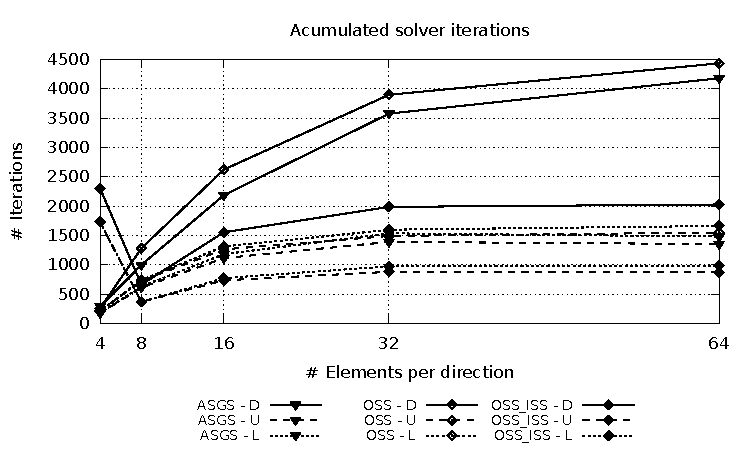
\includegraphics[width=0.49\textwidth]{Figures/Chapter5/colliding/iter}}
  \subfigure[Elapsed CPU time]{\label{fig-CPUtimeU}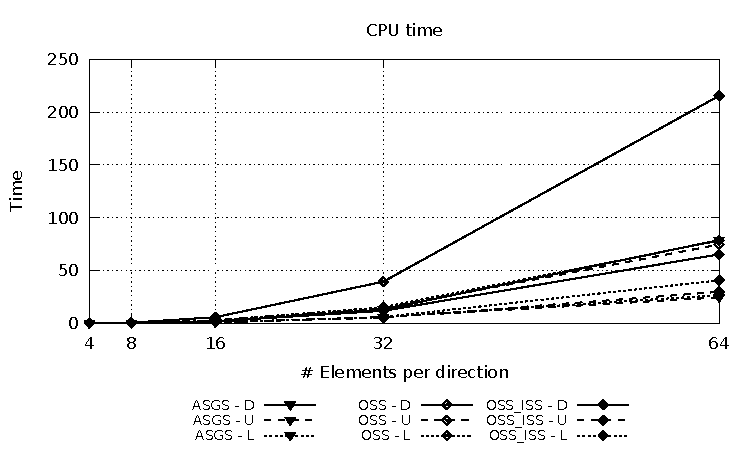
\includegraphics[width=0.49\textwidth]{Figures/Chapter5/colliding/time}}
  \caption{Colliding flow solver iterations and elapsed CPU time using $P_U(\At)$ for the global matrix.}
  \label{fig-soliter-CPUtime}
\end{figure}

Let us now focus on the error in the velocity and pressure fields. Since we are solving a problem with analytical solution, we can evaluate exactly the error of the FE approximation, $e_u:=\|\u_h-\u\|$  and $e_p:=\|p_h-p\|$. \Fig{error} depicts the convergence of both errors when refining the mesh. In \Fig{erroru} we see that the velocity error converges as expected, with a 2nd order rate for the ASGS and OSS methods, which are approximated by $Q_1/Q_1$ elements, and with a 3rd order rate for the OSS-ISS method, which is approximated by a $Q_2/Q_1$ element. 
\begin{figure}[h!]
  \centering
  \subfigure[Velocity error]{\label{fig-erroru}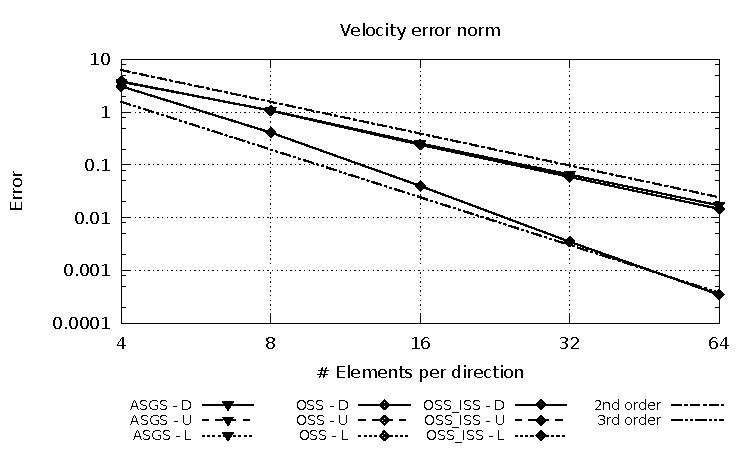
\includegraphics[width=0.49\textwidth]{Figures/Chapter5/colliding/erru}}
  \subfigure[Pressure error]{\label{fig-errorp}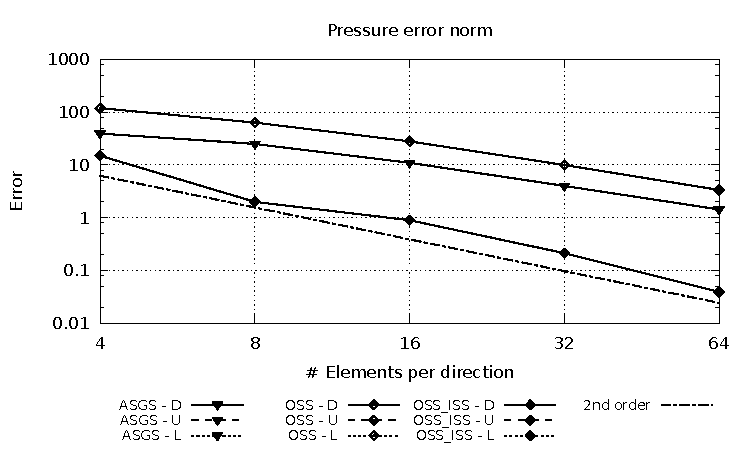
\includegraphics[width=0.49\textwidth]{Figures/Chapter5/colliding/errp}}
  \caption{Colliding flow error convergence using $P_U(\At)$ for the global matrix.}
  \label{fig-error}
\end{figure}
Looking at \Fig{errorp}, it is seen that the pressure error norm converges with a 2nd order rate for all the methods, as expected.
%for the OSS-ISS and a slightly lower rate for the other two cases. 
Note that there is no difference between the results changing the preconditioner, since the solution is the same for all cases because we are not modifying the system that is solved.

In order to check the efficiency of each method we compare the error norm with the elapsed computational time. In this way we have an idea of the time needed for a given method to achieve certain solution accuracy. \Fig{error-time} shows this comparison for velocity (\Fig{erroru-time}) and pressure (\Fig{errorp-time}) fields, where we see that, excluding the coarser mesh, the OSS-ISS method is much more efficient than the other two. Furthermore, the most efficient preconditioner is the upper version $P_U(\K_\tau)$.
\begin{figure}[h!]
  \centering
  \subfigure[Velocity error vs.  CPU time]{\label{fig-erroru-time}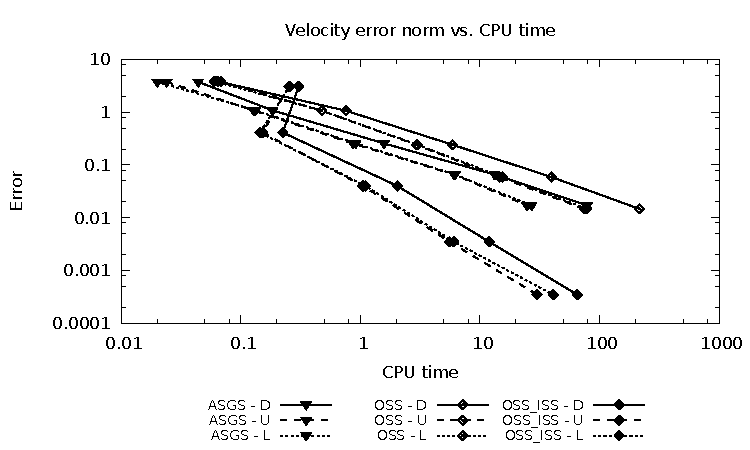
\includegraphics[width=0.49\textwidth]{Figures/Chapter5/colliding/errtu}}
  \subfigure[Pressure error vs.  CPU time]{\label{fig-errorp-time}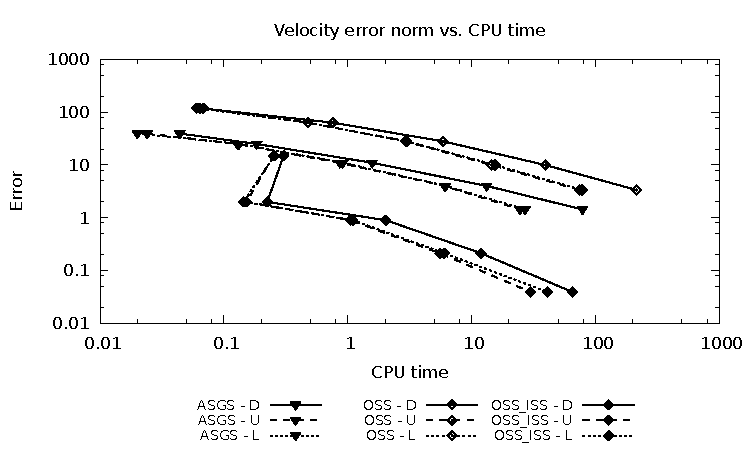
\includegraphics[width=0.49\textwidth]{Figures/Chapter5/colliding/errtp}}
  \caption{Colliding flow error vs. CPU time using $P_U(\At)$ for the global matrix.}
  \label{fig-error-time}
\end{figure}

\subsection{Taylor Green Vortex flow}
\label{subsec-C5_TGV-VMS}
It has been shown by many authors that VMS stabilization terms can act as a LES model for turbulent flows, introducing the appropriate dissipation of the small scales that are not captured by the coarse solution. In particular, ASGS and OSS methods were assessed in \cite{colomes_assessment_2015}, showing that these methods are capable to perform a good LES simulation of different turbulent benchmark problems.
In order to check the performance of the convection-only OSS stabilization of ISS elements for a LES simulation, we analyze its behaviour in the TGV flow, extensively described in Section \ref{subsubsec-C3_TGV}. 

We recall that this test is solved in a computational domain given by the cube $(0,2\pi)^3$ with periodical boundary conditions and the initial condition is given by an analytical field (see, e.g., \cite{brachet_direct_1991})
\begin{align}
\label{eq:ini_sol_TG}
&\u(x,y,z,0)=\left(\begin{array}{c}
u_x\\
u_y\\
u_z
\end{array}\right)=\left(\begin{array}{c}
u_0\cos(x)\sin(y)\sin(z)\\
-u_0\sin(x)\cos(y)\sin(z)\\
0
\end{array}\right)\\\nonumber
&p(x,y,z,0)=p_0+\frac{1}{16}\left(\cos(2x)+\cos(2y)\right)\left(\cos(2z)+2\right),
\end{align}
with
$$u_0=\frac{2}{\sqrt{3}}\sin\left(\gamma+\frac{2\pi}{3}\right).$$
Being $\gamma=0$, resulting in a mean initial velocity  $u_0=1$. We consider the TGV problem with a Reynolds number ${\rm Re}=1600$.

\subsubsection{Setting}
\label{subsubsec-C5_TFV_setting}
The problem is solved from $t=0.0$ to $T=10.0$ with a fixed time step size of $\delta t=5.0\cdot10^{-2}$ using a Crank-Nicolson time integration scheme, and the results are compared against a DNS by Brachet et al. \cite{brachet_direct_1991}. We discretize the domain using different choices of the number of elements and the order of approximation, having two different group of discretizations; one with $32^3$ velocity DOFs and another with $64^3$ velocity DOFs (for each velocity component). The former will be composed by the following meshes: $32^3$ $Q_1/Q_1$, $16^3$ $Q_2/Q_2$ elements or $16^3$ $Q_2/Q_1$ elements when we use ISS discretization. The second group of meshes is made by: $64^3$ $Q_1/Q_1$, $32^3$ $Q_2/Q_2$ or $32^3$ $Q_2/Q_1$ elements. For the stabilized formulations, ASGS and OSS, the algorithmic constants are $c_1=12$ $c_2=2$ and $c_c=0.0$, and for the OSS-ISS method the same $c_1$ and $c_2$ algorithmic constants are used, but $c_c=4.0$ unless noted otherwise. This choice of $c_c$ for the OSS-ISS method is assessed in a following subsection.

\subsubsection{Comparison between VMS methods}
In \Fig{TGV_OSS_32_ene_dis} we show the energy evolution and the energy dissipation rate for the ASGS, the OSS, and the OSS-ISS methods. A first thing that we have to state at this point is that the ASGS method with $32^3$ $Q_1/Q_1$ has failed to converge at early stages of the problem, a behaviour also observed in \cite{colomes_assessment_2015}. Looking at \Fig{TGV_OSS_32_ene} it is clear that the degree of interpolation makes a great difference on the solution, even with the same number of DOFs, the solution is more accurate when a higher order of interpolation is used. In the same figure we see that the loss of precision in the pressure for the ISS elements $Q_2/Q_1$ does affect the solution, giving a result between the $Q_1/Q_1$ and $Q_2/Q_2$ solutions. At \Fig{TGV_OSS_32_dis} we see that the OSS-ISS method is more dissipative than the others. This behaviour is caused by the lack of accuracy in the pressure field, which in turn affects the conservation of mass of the problem. A more exhaustive analysis of the effect of this term is done below.
\begin{figure}[h!]
  \centering
  \subfigure[Energy evolution]{\label{fig-TGV_OSS_32_ene}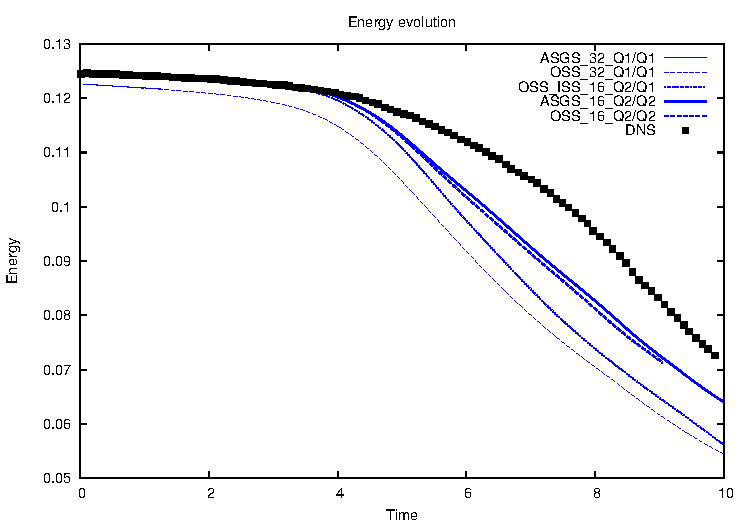
\includegraphics[width=0.49\textwidth]{Figures/Chapter5/TGV/oss_32_ene}}
  \subfigure[Total energy dissipation rate]{\label{fig-TGV_OSS_32_dis}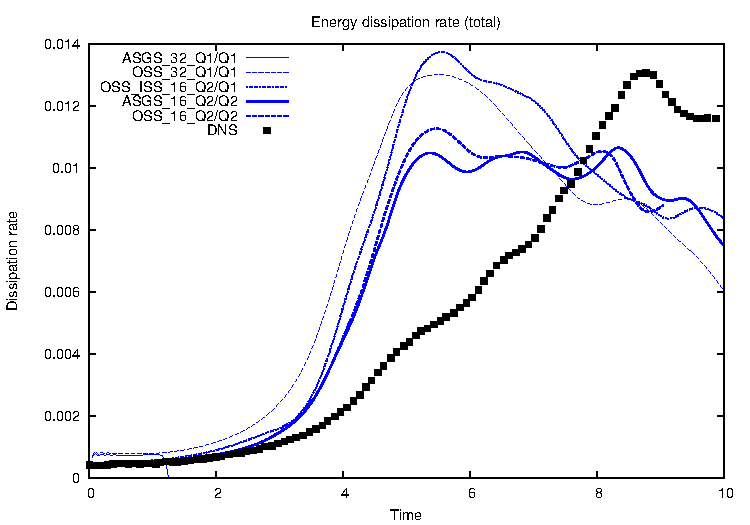
\includegraphics[width=0.49\textwidth]{Figures/Chapter5/TGV/oss_32_tot}}
  \caption{Energy and Total energy dissipation rate evolution with $32^3$ velocity DOFs}
  \label{fig-TGV_OSS_32_ene_dis}
\end{figure}

Although an important improvement of the solution is achieved by increasing the order of interpolation, $32^3$ velocity DOFs is still a very coarse mesh and the results shown in \Fig{TGV_OSS_32_ene_dis} are far from the DNS ones. Then, the same problem is solved in a finer mesh, with the double of velocity DOFs per direction, with the results shown in \Fig{TGV_OSS_64_ene_dis}. In this case, all methods converge at all time steps. \Fig{TGV_OSS_64_ene} depicts the energy evolution and it is also seen that the increase on the degree of interpolation results in a more accurate solution. Both ASGS and OSS methods with $32^3$ $Q_2/Q_2$ elements have very accurate results, providing a solution almost on top of the DNS. There are very little differences between stabilization methods when the same discretization is used. Furthermore, the results of the OSS-ISS method are closer to the $Q_1/Q_1$ discretization than to the $Q_2/Q_2$ one. The total energy dissipation rate shown in \Fig{TGV_OSS_64_dis} denote a very good agreement of the $Q_2/Q_2$ solution with the DNS, while the $Q_1/Q_1$ discretization for both ASGS and OSS methods are still more diffusive. Note that the OSS-ISS method for this discretization has more or less the same energy dissipation as the $Q_1/Q_1$ discretizations.
\begin{figure}[h]
  \centering
  \subfigure[Energy evolution]{\label{fig-TGV_OSS_64_ene}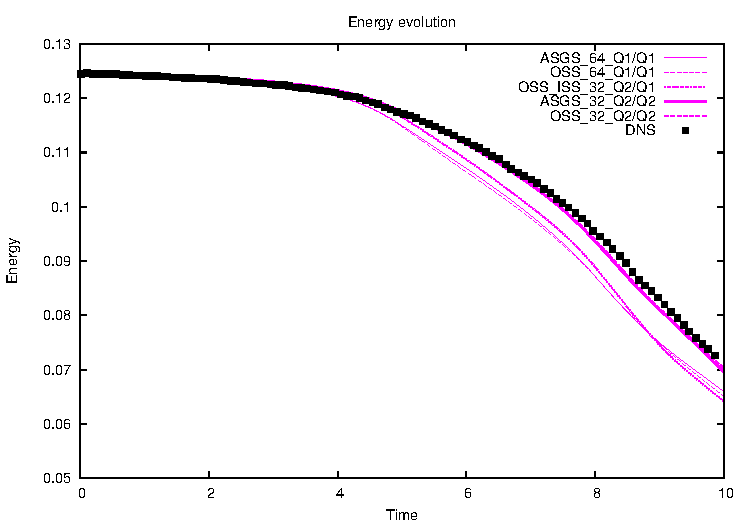
\includegraphics[width=0.49\textwidth]{Figures/Chapter5/TGV/oss_64_ene}}
  \subfigure[Total energy dissipation rate]{\label{fig-TGV_OSS_64_dis}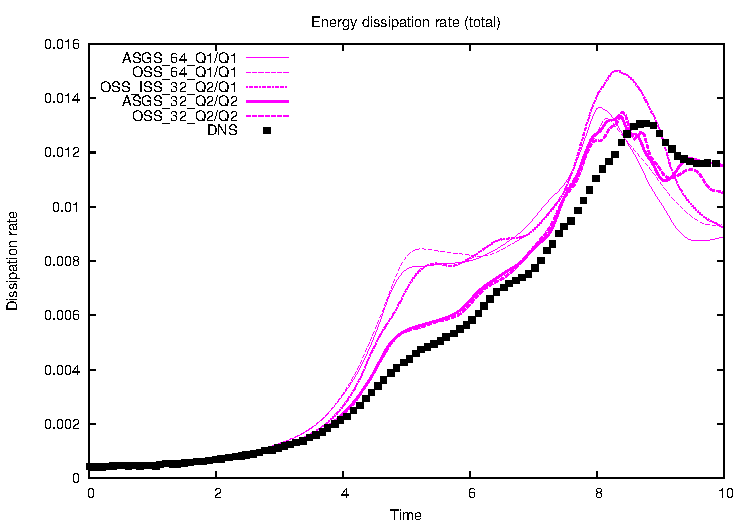
\includegraphics[width=0.49\textwidth]{Figures/Chapter5/TGV/oss_64_tot}}
  \caption{Energy and Total energy dissipation rate evolution with $64^3$ velocity DOFs}
  \label{fig-TGV_OSS_64_ene_dis}
\end{figure}

When analyzing the suitability of a LES model, a very important turbulent quantity to take into account is the energy spectra. It gives us information about how the energy is distributed among the scales of the problem. In order to assess the behaviour of the proposed methods in that aspect, we compare our results by the DNS by Gassner et al. \cite{gassner_accuracy_2013}. In \Fig{TGV_OSS_spe} the energy spectra at $t=9.0$ is depicted for both discretization groups. The coarser cases shown in \Fig{TGV_OSS_32_spe} are all far from the DNS result, but follow the same pattern, with most of the energy on the greatest scales and little energy on the small scales, without any pileup of energy on the small scales. When the mesh is refined, see \Fig{TGV_OSS_64_spe}, the computed energy spectra tends to the DNS one. Note that also in this plot, $Q_2/Q_2$ discretization have better agreement with the DNS, specially on the small scales, where the influence of the enrichment of the interpolation space is patent.
\begin{figure}[h]
  \centering
  \subfigure[$32^3$ velocity DOFs]{\label{fig-TGV_OSS_32_spe}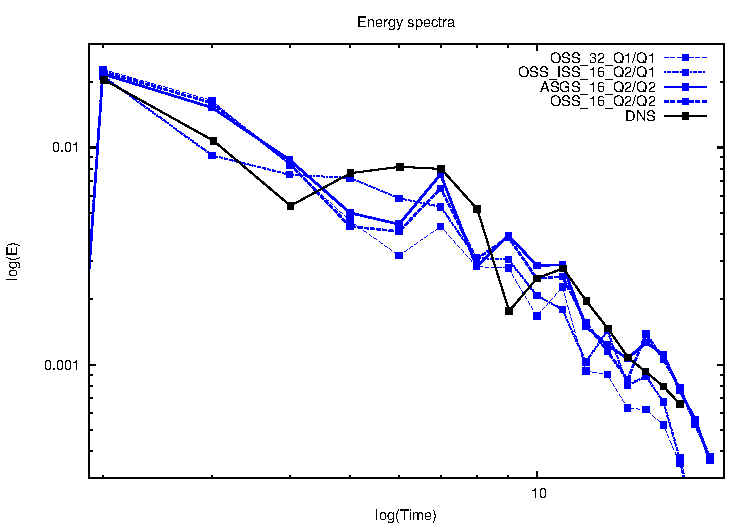
\includegraphics[width=0.49\textwidth]{Figures/Chapter5/TGV/oss_32_spe}}
  \subfigure[$64^3$ velocity DOFs]{\label{fig-TGV_OSS_64_spe}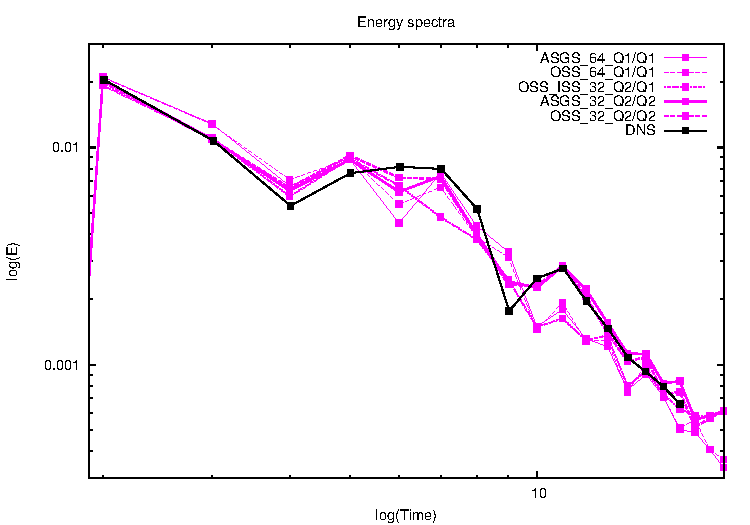
\includegraphics[width=0.49\textwidth]{Figures/Chapter5/TGV/oss_64_spe}}
  \caption{Energy spectra at $t=9.0$}
  \label{fig-TGV_OSS_spe}
\end{figure}

\subsubsection{Computational cost}
It is clear that a good LES model has to reproduce as accurately as possible all the turbulent quantities, even for coarse meshes. The results presented until now show that ASGS and OSS methods perform better than the OSS-ISS when $Q_2/Q_2$ elements are used. Additionally, it has been seen that all methods converge to the DNS results when the mesh is refined. But a crucial point that has to be always taken into account when we talk about numerical simulations is the computational cost. At the end, we are looking for the cheapest method that allow us to reproduce accurately the physical phenomena that takes place in a turbulent flow. So in this subsection we will discuss the computational cost associated to each method and their efficiency when solving this kind of flows.

To check the computational cost we look at the number of solver iterations needed for each method, shown in \Fig{TGV_OSS_iter}. In particular, \Fig{TGV_OSS_iter_ite} depicts the total amount of solver iterations at each time step, adding up all nonlinear iterations. Note that the change of the nonlinear iterations along the time can be clearly noticed by the jumps on the curves. We see that the cheapest method is the OSS-ISS for both discretizations, $32^3$ and $64^3$ velocity DOFs, with much less solver iterations per time step than the other methods. It is also seen that ASGS is a little bit cheaper than the OSS method, which can be caused by the size of the system, much bigger for the OSS case due to the implicit treatment of the projections. An interesting result also seen in \ref{fig-TGV_OSS_iter_ite} is the improvement on the computational cost when we go from $Q_1/Q_1$ to $Q_2/Q_2$ discretization, keeping constant the number of DOFs.
\begin{figure}[h!]
  \centering
  \subfigure[Solver iterations per time step]{\label{fig-TGV_OSS_iter_ite}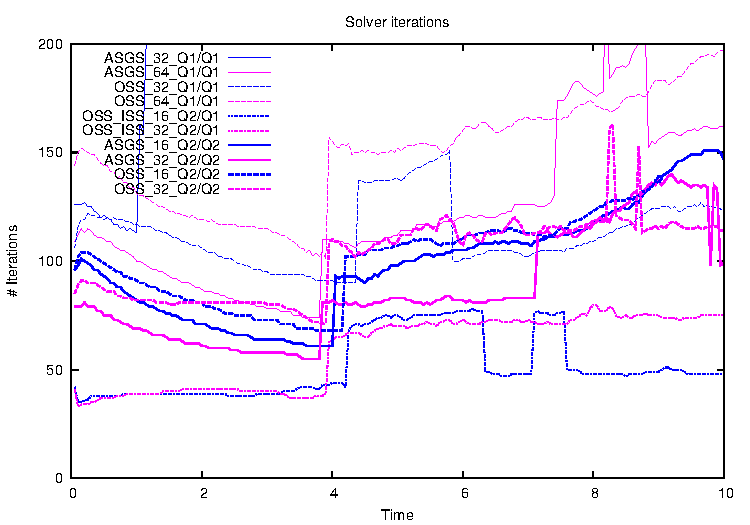
\includegraphics[width=0.49\textwidth]{Figures/Chapter5/TGV/oss_all_ite}}
  \subfigure[Accumulated solver iterations]{\label{fig-TGV_OSS_iter_acu}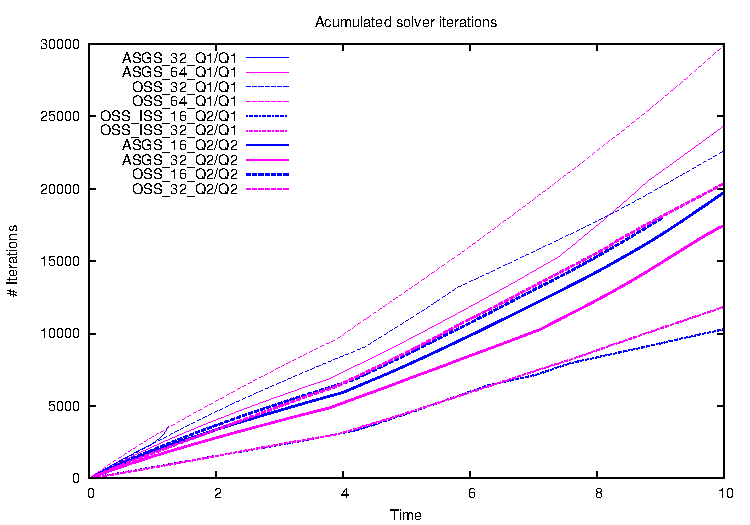
\includegraphics[width=0.49\textwidth]{Figures/Chapter5/TGV/oss_all_acu}}
  \caption{Computational cost}
  \label{fig-TGV_OSS_iter}
\end{figure}
Looking at \ref{fig-TGV_OSS_iter_acu} we realize that at the end of the computation, the total amount of solver iterations needed by OSS-ISS method is around 1.5 times less than the ASGS method, for the finer mesh, and half of them for the coarse mesh. This result indicates that the OSS-ISS is a very good approach as a LES model for turbulent problems since, although it has been seen that is not the most accurate when looking to the turbulent quantities, it is much cheaper and we can refine the mesh in order to get better results remaining competitive with the other methods. Further, let us remark that the pressure Poisson solvers are the most computationally intensive, and ISS methods involve $Q_1$ pressure spaces for $Q_2$ ones for stabilized methods.

\subsubsection{Influence of the pressure subscale term}
As said above and also stated in Section \ref{subsec-C5_pressure_subscale}, the pressure subscale $\tau_c(\nabla\cdot\u_h,\nabla\cdot\v_h)$ term has an important role when using ISS elements. In this subsection we are going to analyse the effect of this term on the results when simulating the TGV problem. Hence, we redefine the $\tau_c$ definition in \Eq{C2_tau_c} by
\begin{equation}
\label{eq-C5_tau_c_2}
\tau_c=c_c\left(\nu+\frac{c_2}{c_1}h|\u_h|\right),
\end{equation}
which is equivalent to \Eq{C2_tau_c} when $c_c=1.0$. We keep the algorithmic parameters $c1=12.0$ and $c2=2.0$ constant, so considering different values of $c_c$ we can evaluate the influence of the pressure subscale term on the solution. In this case we choose six different configurations $c_c=\{0.0,0.25,0.5,1.0,2.0,4.0\}$ and solve the problem with the $16^3$ $Q_2/Q_1$ elements mesh. We compare the solution against the one obtained with the OSS method with $16^3$ $Q_2/Q_2$ elements discretization. 
%In this test, a second order SRK scheme with explicit time integration of the convective term has been used to solve the problem, with a time step size of $\delta t=5.0\cdot10^{-2}$. The main goal of a SRK scheme is the velocity and pressure decoupling, allowing the use of more efficient solvers.

In \Fig{TGV_OSS_tauc_vis} the energy dissipation rate of the FE counterpart is shown. That is the viscous term $\nu\|\nabla\u_h\|^2$ that appears in equation \Eq{C5_ene_total}. We see that when we reduce $c_c$ the viscous dissipation introduced by the FE counterpart increase, being the case $ c_c=0.5 $ the one closer to the DNS curve.
%the method becomes more dissipative and it may seem a good idea to keep this term as small as possible in order to get closer to the DNS curve. 
But if we look at the energy spectra shown in \Fig{TGV_OSS_tauc_spe}, we see that this is not a good choice. What is actually happening when $c_c$ goes to zero is that the dissipation is taking place in the largest scales of the problem, while the smallest ones keep the energy, resulting in an energy pileup at the tail of the spectra. This means that the energy is not dissipating in the correct way and the small scales, which are the ones that have more influence on the viscous dissipation term, have more energy than the desired one. Therefore, a good selection is to choose $c_c=4.0$, which results are closer to the OSS method and has a better energy spectra shape. A higher value of $c_c$ eventually lead to unstable solutions, for instance, with $c_c=8.0$ and $\delta t=5.0\cdot10^{-2}$ the solution fails to converge at $t=0.4$. In that case, the solution becomes unstable and the nonlinear iteratition does not reach the required tolerance.
\begin{figure}[h!]
  \centering
  \subfigure[Viscous energy dissipation rate]{\label{fig-TGV_OSS_tauc_vis}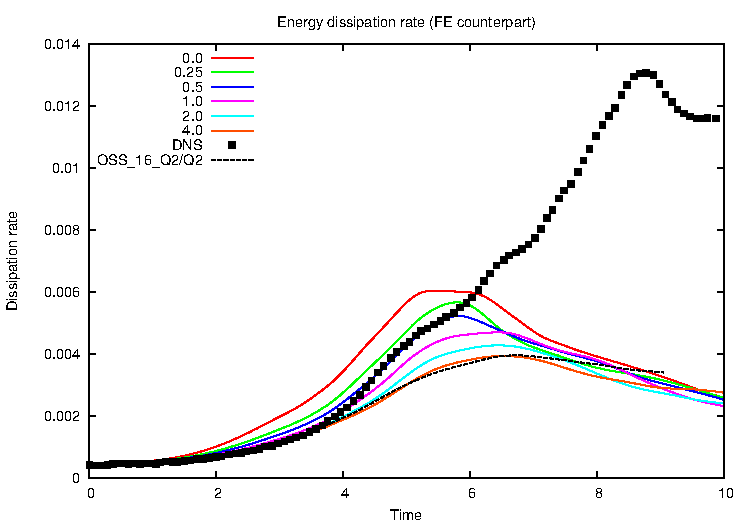
\includegraphics[width=0.49\textwidth]{Figures/Chapter5/TGV/oss_ktc_vis}}
  \subfigure[Energy spectra]{\label{fig-TGV_OSS_tauc_spe}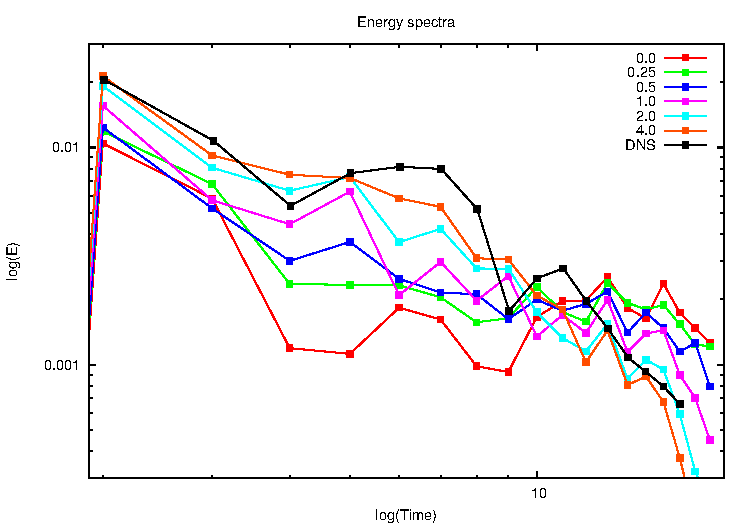
\includegraphics[width=0.49\textwidth]{Figures/Chapter5/TGV/oss_ktc_spe}}
  \caption{Comparison for different $c_c$ choices for OSS-ISS with $32^3$ velocity DOFs}
  \label{fig-TGV_OSS_tauc}
\end{figure}

As stated in Section \ref{subsec-C5_pressure_subscale}, the pressure subscale term is essential to enforce the incompressibility constrain at the discrete level. In \Fig{TGV_OSS_tauc_divvel} the total energy dissipation rate (\Fig{TGV_OSS_tauc_dis}) is depicted together with the velocity divergence $L2$-norm $\|\nabla\cdot\u_h\|$ (\Fig{TGV_OSS_tauc_div}). We see that, effectively, $\|\nabla\cdot\u_h\|$ is reduced when $\tau_c$ is increased. The case of $c_c=0.0$ give especially bad results in terms of mass conservation, affecting also to the energy dissipation rate. In this case, as seen in \Fig{TGV_OSS_tauc_spe}, the over-dissipation on the large scales and the under-dissipation on the smallest ones makes that the velocity spatial derivatives become relevant, increasing the $\|\nabla\cdot\u_h\|$ term. The introduction of $\tau_c\|\nabla\cdot\u_h\|$ into the energy dissipation equation \Eq{C5_ene_total} changes the way in which the flow dissipates its energy among the different scales, decreasing the energy of the small scales and, then, reducing the importance of the spatial derivatives, which is reflected in a lower value of $\|\nabla\cdot\u_h\|$ but also in a lower dissipation rate, as seen in \Fig{TGV_OSS_tauc_dis}, even if a positive term has been added to \Eq{C5_ene_total}.
\begin{figure}[h!]
  \centering
  \subfigure[Total energy dissipation rate]{\label{fig-TGV_OSS_tauc_dis}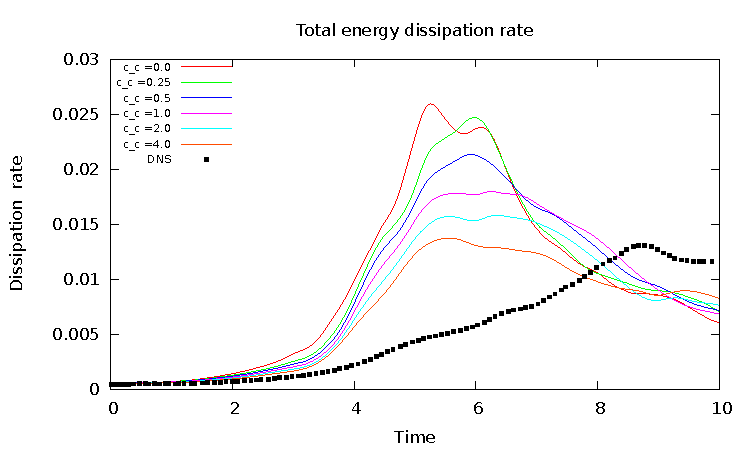
\includegraphics[width=0.49\textwidth]{Figures/Chapter5/TGV/srk_ktc_32_dis}}
  \subfigure[$\|\nabla\cdot\u_h\|$]{\label{fig-TGV_OSS_tauc_div}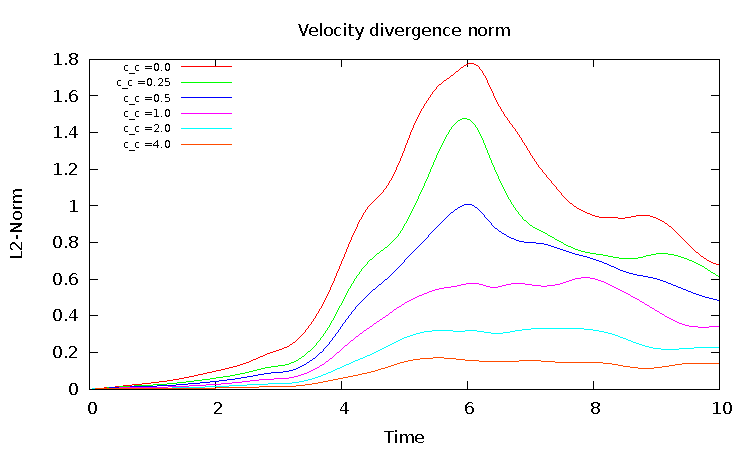
\includegraphics[width=0.49\textwidth]{Figures/Chapter5/TGV/srk_ktc_32_divvel}}
  \caption{Total energy dissipation and velocity divergence $L2$-norm for different $c_c$ choices for OSS-ISS with $32^3$ velocity DOFs}
  \label{fig-TGV_OSS_tauc_divvel}
\end{figure}

\subsubsection{Refinement analysis for the OSS-ISS method}
In the computational cost analysis shown above we have seen that OSS-ISS has a great potential as a LES model, especially when we the computational cost is taken into account. This subsection aims to check the performance of this method when we refine the mesh both reducing the element size and increasing the interpolation order. 
%As done in previous subsection the time integration technique used in these tests is the Segregated Runge-Kutta method.

Once determined that the best algorithmic constant for the pressure subscale term is $c_c=4.0$ when ISS FEs are used, we keep this value constant and change the discretization. A refinement analysis can be done to determine if the LES approach presented in this work effectively converges to the DNS solution when we refine the mesh. In section \ref{subsec-C5_TGV-VMS} the TGV problem has been solved using different discretizations with $32^3$ and $64^3$ velocity DOFs. Now we go further and also solve the problem with $96^3$ velocity DOFs, that is a $48^3$ $Q_2/Q_1$ elements mesh. Furthermore, here we also use $Q_3/Q_2$ FEs. In particular, a $21^3$ and $32^3$ $Q_3/Q_2$ elements meshes are used, corresponding to the group of $64^3$ and $96^3$ velocity DOFs, respectively. We also decrease the time step to $\delta t=2.5\cdot10^{-2}$ for the discretizations with $64^3$ velocity DOFs and $\delta t=1.5\cdot10^{-2}$ for the discretizations with $96^3$ velocity DOFs.

In \Fig{TGV_OSS_tauc_refinement} we depict the kinetic energy and the total energy dissipation rate evolution for the different discretizations considered in this refinement analysis. Looking at the energy evolution in \Fig{TGV_OSS_tauc_refinement_ene} it is clearly seen that the solution converge to the DNS results, giving the $32^3$ $Q_3/Q_2$ elements mesh a very accurate solution, which is also evident in \Fig{TGV_OSS_tauc_refinement_dis} where the total energy dissipation rate of this discretization is on top of the DNS solution. We also see in \Fig{TGV_OSS_tauc_refinement} the relevance of the degree of interpolation, where for a given number of DOFs, the higher-order discretization results in a better solution.
\begin{figure}[h]
  \centering
  \subfigure[Energy evolution]{\label{fig-TGV_OSS_tauc_refinement_ene}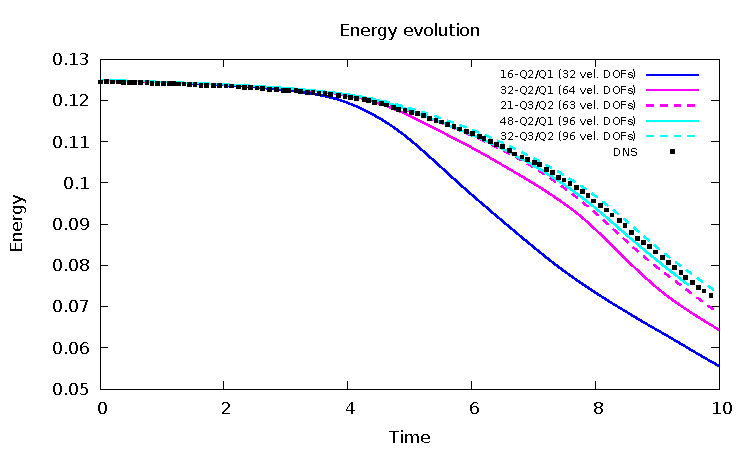
\includegraphics[width=0.49\textwidth]{Figures/Chapter5/TGV/srk_ktc_ene}}
  \subfigure[Total energy dissipation rate]{\label{fig-TGV_OSS_tauc_refinement_dis}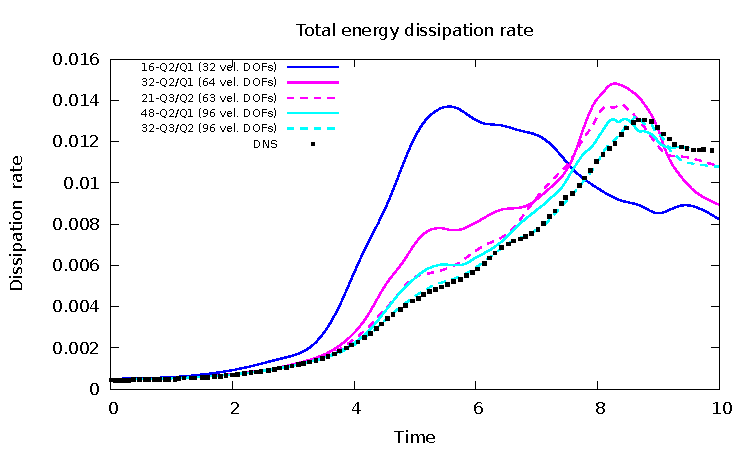
\includegraphics[width=0.49\textwidth]{Figures/Chapter5/TGV/srk_ktc_dis}}
  \caption{Energy and Total energy dissipation rate evolution refining the mesh with $c_c=4.0$.}
  \label{fig-TGV_OSS_tauc_refinement}
\end{figure}

Now, we ask ourselves how the tuning of the parameter $\tau_c$ affects when finer meshes are used. In particular, we want to know how important the $c_c$ parameter becomes when higher order FEs are used. To answer this question we solve the TGV problem for two different discretizations: $32^3$ $Q_2/Q_1$ and $21^3$ $Q_3/Q_2$ elements meshes, and three different values of $c_c$: $0.0$, $1.0$ and $4.0$.

\begin{figure}[h!]
  \centering
  \subfigure[Total energy dissipation rate]{\label{fig-TGV_OSS_refinement_tauc_dis}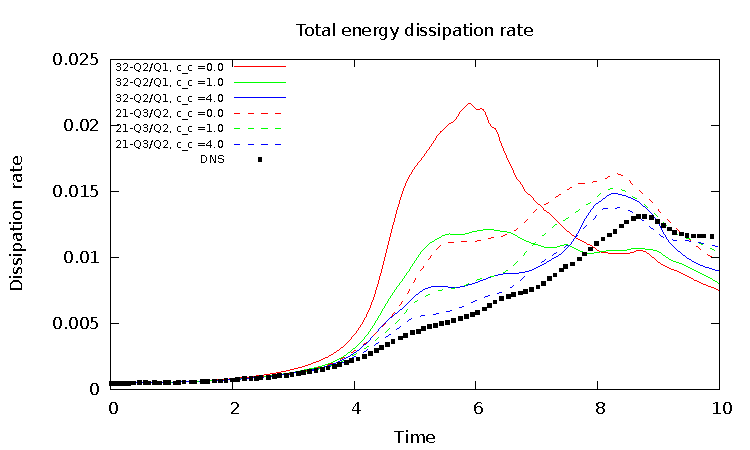
\includegraphics[width=0.49\textwidth]{Figures/Chapter5/TGV/srk_ktc_64_dis}}
  \subfigure[$\|\nabla\cdot\u_h\|$]{\label{fig-TGV_OSS_refinement_tauc_div}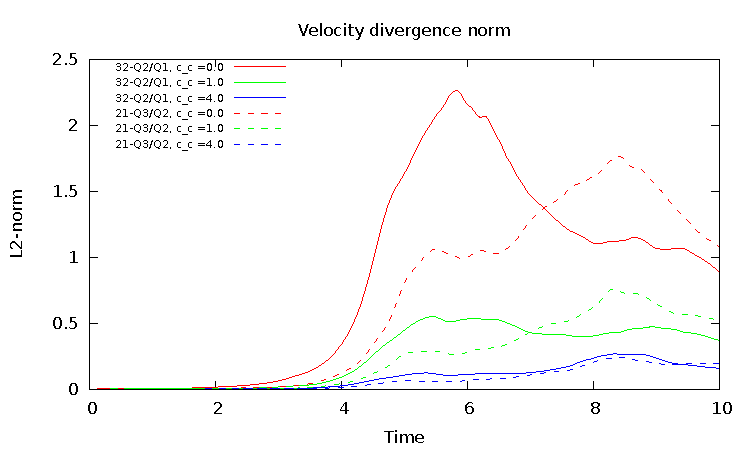
\includegraphics[width=0.49\textwidth]{Figures/Chapter5/TGV/srk_ktc_64_divvel}}
  \caption{Total energy dissipation and velocity divergence $L2$-norm for different $c_c$ choices for OSS-ISS with $64^3$ velocity DOFs}
  \label{fig-TGV_OSS_refinement_tauc_divvel}
\end{figure}
\Fig{TGV_OSS_refinement_tauc_divvel} depicts the total energy dissipation rate (\Fig{TGV_OSS_refinement_tauc_dis})  and the velocity divergence $L2$-norm (\Fig{TGV_OSS_refinement_tauc_div}) for the two discretizations considered and for different choices of $c_c$. We still see a dependence on $c_c$, but differences reduce when higher order of interpolation is used, as expected. It is also seen that when increasing $c_c$, the differences between the two discretizations are reduced (for a fixed $c_c$). This behaviour is particularly significant when we look at the velocity divergence norm in \Fig{TGV_OSS_refinement_tauc_div}, where we see that for $c_c=0$ the two discretizations give a completely different evolution of $\|\nabla\cdot\u_h\|$, while for $c_c=4.0$ the results are almost the same. In the same figure, we can see that the largest value of $\|\nabla\cdot\u_h\|$ for $c_c$ is larger than the largest one depicted in \Fig{TGV_OSS_tauc_div}, which is a result of a $16^3$ $Q_2/Q_1$ elements mesh. 

Going further we also do the same test for the $48^3$ $Q_2/Q_1$ and $32^3$ $Q_3/Q_2$ elements mesh (\Fig{TGV_OSS_refinement_tauc_divvel_96}). In this figure we see that the differences between the three $c_c$ cases are reduced. Looking at \Fig{TGV_OSS_refinement_tauc_dis_96} it is seen that for $c_c=0$ and $Q_2/Q_1$ elements, although the result is far from the DNS, the maximum value of the dissipation rate is much lower than the given in \Fig{TGV_OSS_refinement_tauc_dis}. When using $Q_3/Q_2$ elements, the changes on $c_c$ produce lower differences compared against the $Q_2/Q_1$ approximation. The divergence norm depicted in \Fig{TGV_OSS_refinement_tauc_divvel_96} also show improvements with respect to \Fig{TGV_OSS_refinement_tauc_divvel}. In this case, the maximum value of the divergence for $c_c$ for $Q_2/Q_1$ elements is lower than the case of $64^3$ velocity DOFs and also for the case of $32^3$ velocity DOFs.
\begin{figure}[h!]
  \centering
  \subfigure[Total energy dissipation rate]{\label{fig-TGV_OSS_refinement_tauc_dis_96}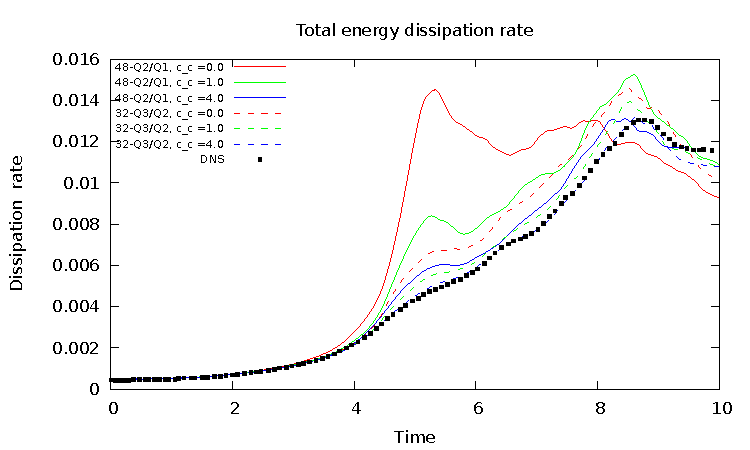
\includegraphics[width=0.49\textwidth]{Figures/Chapter5/TGV/srk_ktc_96_dis}}
  \subfigure[$\|\nabla\cdot\u_h\|$]{\label{fig-TGV_OSS_refinement_tauc_div_96}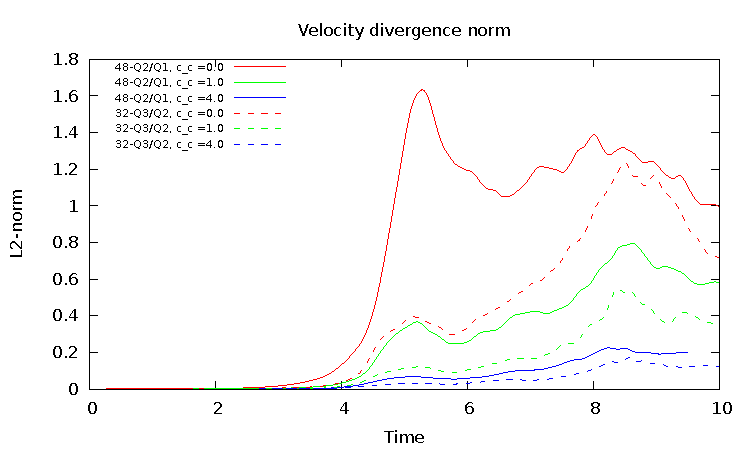
\includegraphics[width=0.49\textwidth]{Figures/Chapter5/TGV/srk_ktc_96_divvel}}
  \caption{Total energy dissipation and velocity divergence $L2$-norm for different $c_c$ choices for OSS-ISS with $96^3$ velocity DOFs}
  \label{fig-TGV_OSS_refinement_tauc_divvel_96}
\end{figure}

To summarize, we have checked that refining the mesh we converge to the DNS results and, for a given number of DOFs, the results improve when higher order interpolation is used. On the hand, we have seen that increasing $c_c$ we reduce $\|\nabla\cdot\u\|$, and consequently the accuracy of the solution. %Furthermore, the difference on the results changing $c_c$ is smaller when we refine the mesh, and for a given amount of DOFs, this difference is still lower when higher order interpolations are used.

\subsection{Turbulent channel flow at $Re_\tau=395$}
\label{subsec-C5_turb_channel}
In Section \ref{subsec-C5_TGV-VMS} we have tested an homogeneous turbulent flow. Now, we want to check the behaviour of the proposed OSS-ISS stabilization method for a wall bounded turbulent test. To do so, we use the Turbulent Channel Flow test with a Reynolds number based on the wall friction ($Re_\tau$) equal to 395. This benchmark was exhaustively tested using a VMS method with OSS in previous \Chap{Rb_VMS}.

\subsubsection{Setting}
Recalling the problem description exposed in Section \ref{subsubsec-C3_TCF}, the domain of the TCF problem for $Re_\tau=395$ is given by a box of length $(2\pi\delta\times 2\delta\times 2/3\pi\delta)$. The $x$-direction is the flow direction, also called stream-wise direction, the $y$-direction is the wall-normal direction, and the $z$-direction is the span-wise direction. Homogeneous Dirichlet boundary conditions for the velocity DOFs are imposed on wall-normal direction boundaries ($y=-\delta$ and $y=\delta$), while periodic boundary conditions are defined on the stream-wise and span-wise directions.

The problem is solved using two different meshes, with $32^3$ $Q_2-Q_1$ and $21^3$ $Q_3/Q_2$ elements mesh. Both meshes have refined elements near the wall in the wall-normal direction, like the one used in \cite{colomes_assessment_2015}. The algorithmic constants that appear in the OSS-ISS method will be discussed in the following subsections.

The obtained results are compared against a DNS computed in \cite{moser_direct_1999,kim_turbulence_1987} (MKM-DNS), then, the parameter election will be according to the ones defined in the cited paper. The bulk mean velocity and the half channel height are taken equal to one, $\bar{U}=1$ and $\delta=1$. Knowing the estimated Reynolds number based on the bulk mean velocity, $Re=\bar{U}2\delta/\nu\approx 13,750$ (see \cite{pope_turbulent_2000}), one can obtain the value of the viscosity, $\nu=1.4545\cdot10^{-4}$. From the Reynolds number based on the friction velocity, we can determine the friction velocity magnitude: $u_\tau=Re_\tau\nu/\delta=5.745\cdot10^{-2}$. Thus, the wall shear stress reads $\tau_w=u_\tau^2=3.3010\cdot10^{-3}$. A force equivalent to a pressure gradient is imposed to drive the movement of the flow in the stream-wise direction, $f_x=\tau_w/\delta$.

In order to achieve the statistically steady state solution, an initial solution is provided following \cite{moin_numerical_1980}. This initial solution consists in a unidirectional velocity profile over which is added a fluctuation:
\begin{align}
\label{eq-C5_TCF_initial_sol}
&u_x = C\left(1-y^8\right)+\epsilon\frac{L_x}{2}\sin(\pi y)\cos\left(\frac{4\pi x}{L_x}\right)\sin\left(\frac{2\pi z}{L_z}\right),\\\nonumber
&u_y = -\epsilon(1+\cos(\pi y))\sin(\pi y)\sin\left(\frac{4\pi x}{L_x}\right)\sin\left(\frac{2\pi z}{L_z}\right),\\
&u_z = -\epsilon\frac{L_z}{2}\sin\left(\frac{4\pi x}{L_x}\right)\sin(\pi y)\cos\left(\frac{2\pi z}{L_z}\right).\nonumber
\end{align}
The constant $C$ is chosen in such a way that the field without fluctuations would have a bulk mean velocity $\bar{U}=1.0$. The fluctuation constant $\epsilon$ is $10\%$ of the bulk mean velocity.

\subsubsection{Effect of the pressure subscale term on the conservation of mass}
As it has been said in Section \ref{subsec-C5_pressure_subscale}, the pressure subscale term has a noticeable effect on the solution when ISS elements are used. The effect of this term has also been analyzed in a previous test, see Section \ref{subsec-C5_TGV-VMS}. Here we will also assess the effect of this term on a wall-bounded flow.

First we will focus on the effect of the second term in \Eq{C5_tau_c_2}, looking how the $c_2/c_1$ ratio affects the solution keeping $c_c=1.0$. As we are in a turbulent regime, we do not expect that the viscous counterpart in \Eq{C2_tau_m} will have relevance on the solution, but we do expect it for the convective counterpart. Then, we will keep $c_1=12.0$ and we will increase $c_2$ from $1.0$ to $16.0$. The variations on $c_2$ not only have an effect on $\tau_c$ but also on $\tau_m$. We solve the problem from $t=0$ to $t=20\pi$ (time needed to cross the channel 10 times, based on the initial mean bulk velocity $\bar{U}$) starting from the initial solution \Eq{C5_TCF_initial_sol} using the implicit version of \textit{(3-3)} SRK scheme. The energy and $\|\nabla\cdot\u_h\|$ evolution are plotted in \Fig{cha_c2}.
\begin{figure}[h!]
  \centering
  \subfigure[Energy evolution]{\label{fig-cha_c2_ene}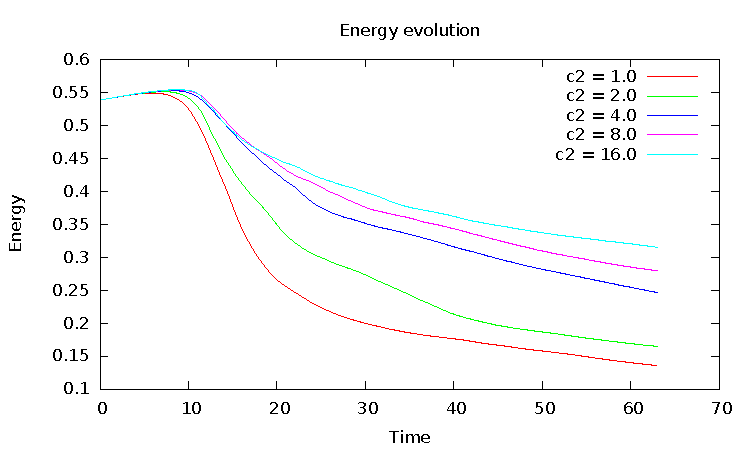
\includegraphics[width=0.49\textwidth]{Figures/Chapter5/TCF/divergence/ktau2/ene}}
  \subfigure[$\|\nabla\cdot\u_h\|$]{\label{fig-cha_c2_div}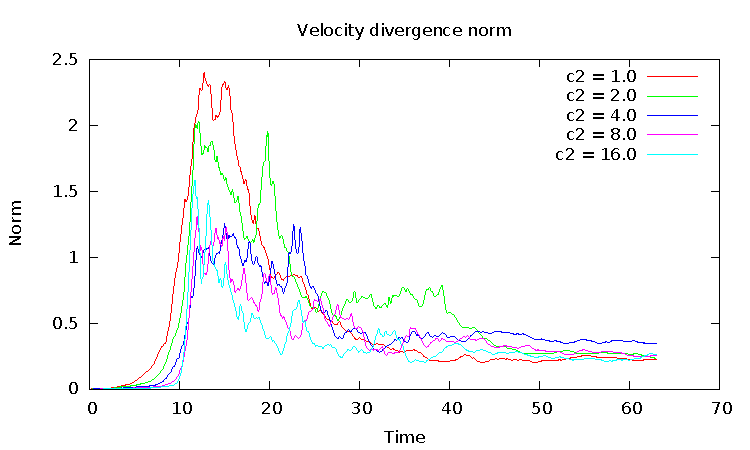
\includegraphics[width=0.49\textwidth]{Figures/Chapter5/TCF/divergence/ktau2/divel}}
  \caption{Energy evolution and velocity divergence norm for different values of $c_2$, keeping $c_1=12.0$ and $c_c=1.0$}
  \label{fig-cha_c2}
\end{figure}
It is clearly seen in \Fig{cha_c2} that the modification of $c_2$ has an effect on the solution. We see in \Fig{cha_c2_ene} that the energy drops faster when lower values of $c_2$ are used. Looking at \Fig{cha_c2_div} we see that the velocity divergence $L_2$-norm is higher when lower values of $c_2$ are taken. The evolution of $\|\nabla\cdot\u_h\|$ gives us information about how the flow is evolving. From an initial and structured condition, the flow starts becoming chaotic around $t=10$, depending on the case, when the turbulent structures increase the rotation of the flow particles, growing the spatial derivatives. At this stage, the energy dissipates until the equilibrium between the internal energy and the external forces is reached. These stages can be seen in \Fig{cha_c2_1.0_vel}, where we depict the vorticity isosurfaces for $|\omega|=5.0$ coloured with the velocity field module at $t=0.15$ (\Fig{cha_c2_1.0_vel_1.0}),  at $t=12.0$ (\Fig{cha_c2_1.0_vel_12.0}) and at $t=70.0$ (\Fig{cha_c2_1.0_vel_60.0}) setting $c2=1.0$ and $c_c=32.0$, and using a $32^3$ $Q_2/Q_1$ elements mesh.
\begin{figure}[h!]
  \centering
  \subfigure[$t=0.15$]{\label{fig-cha_c2_1.0_vel_1.0}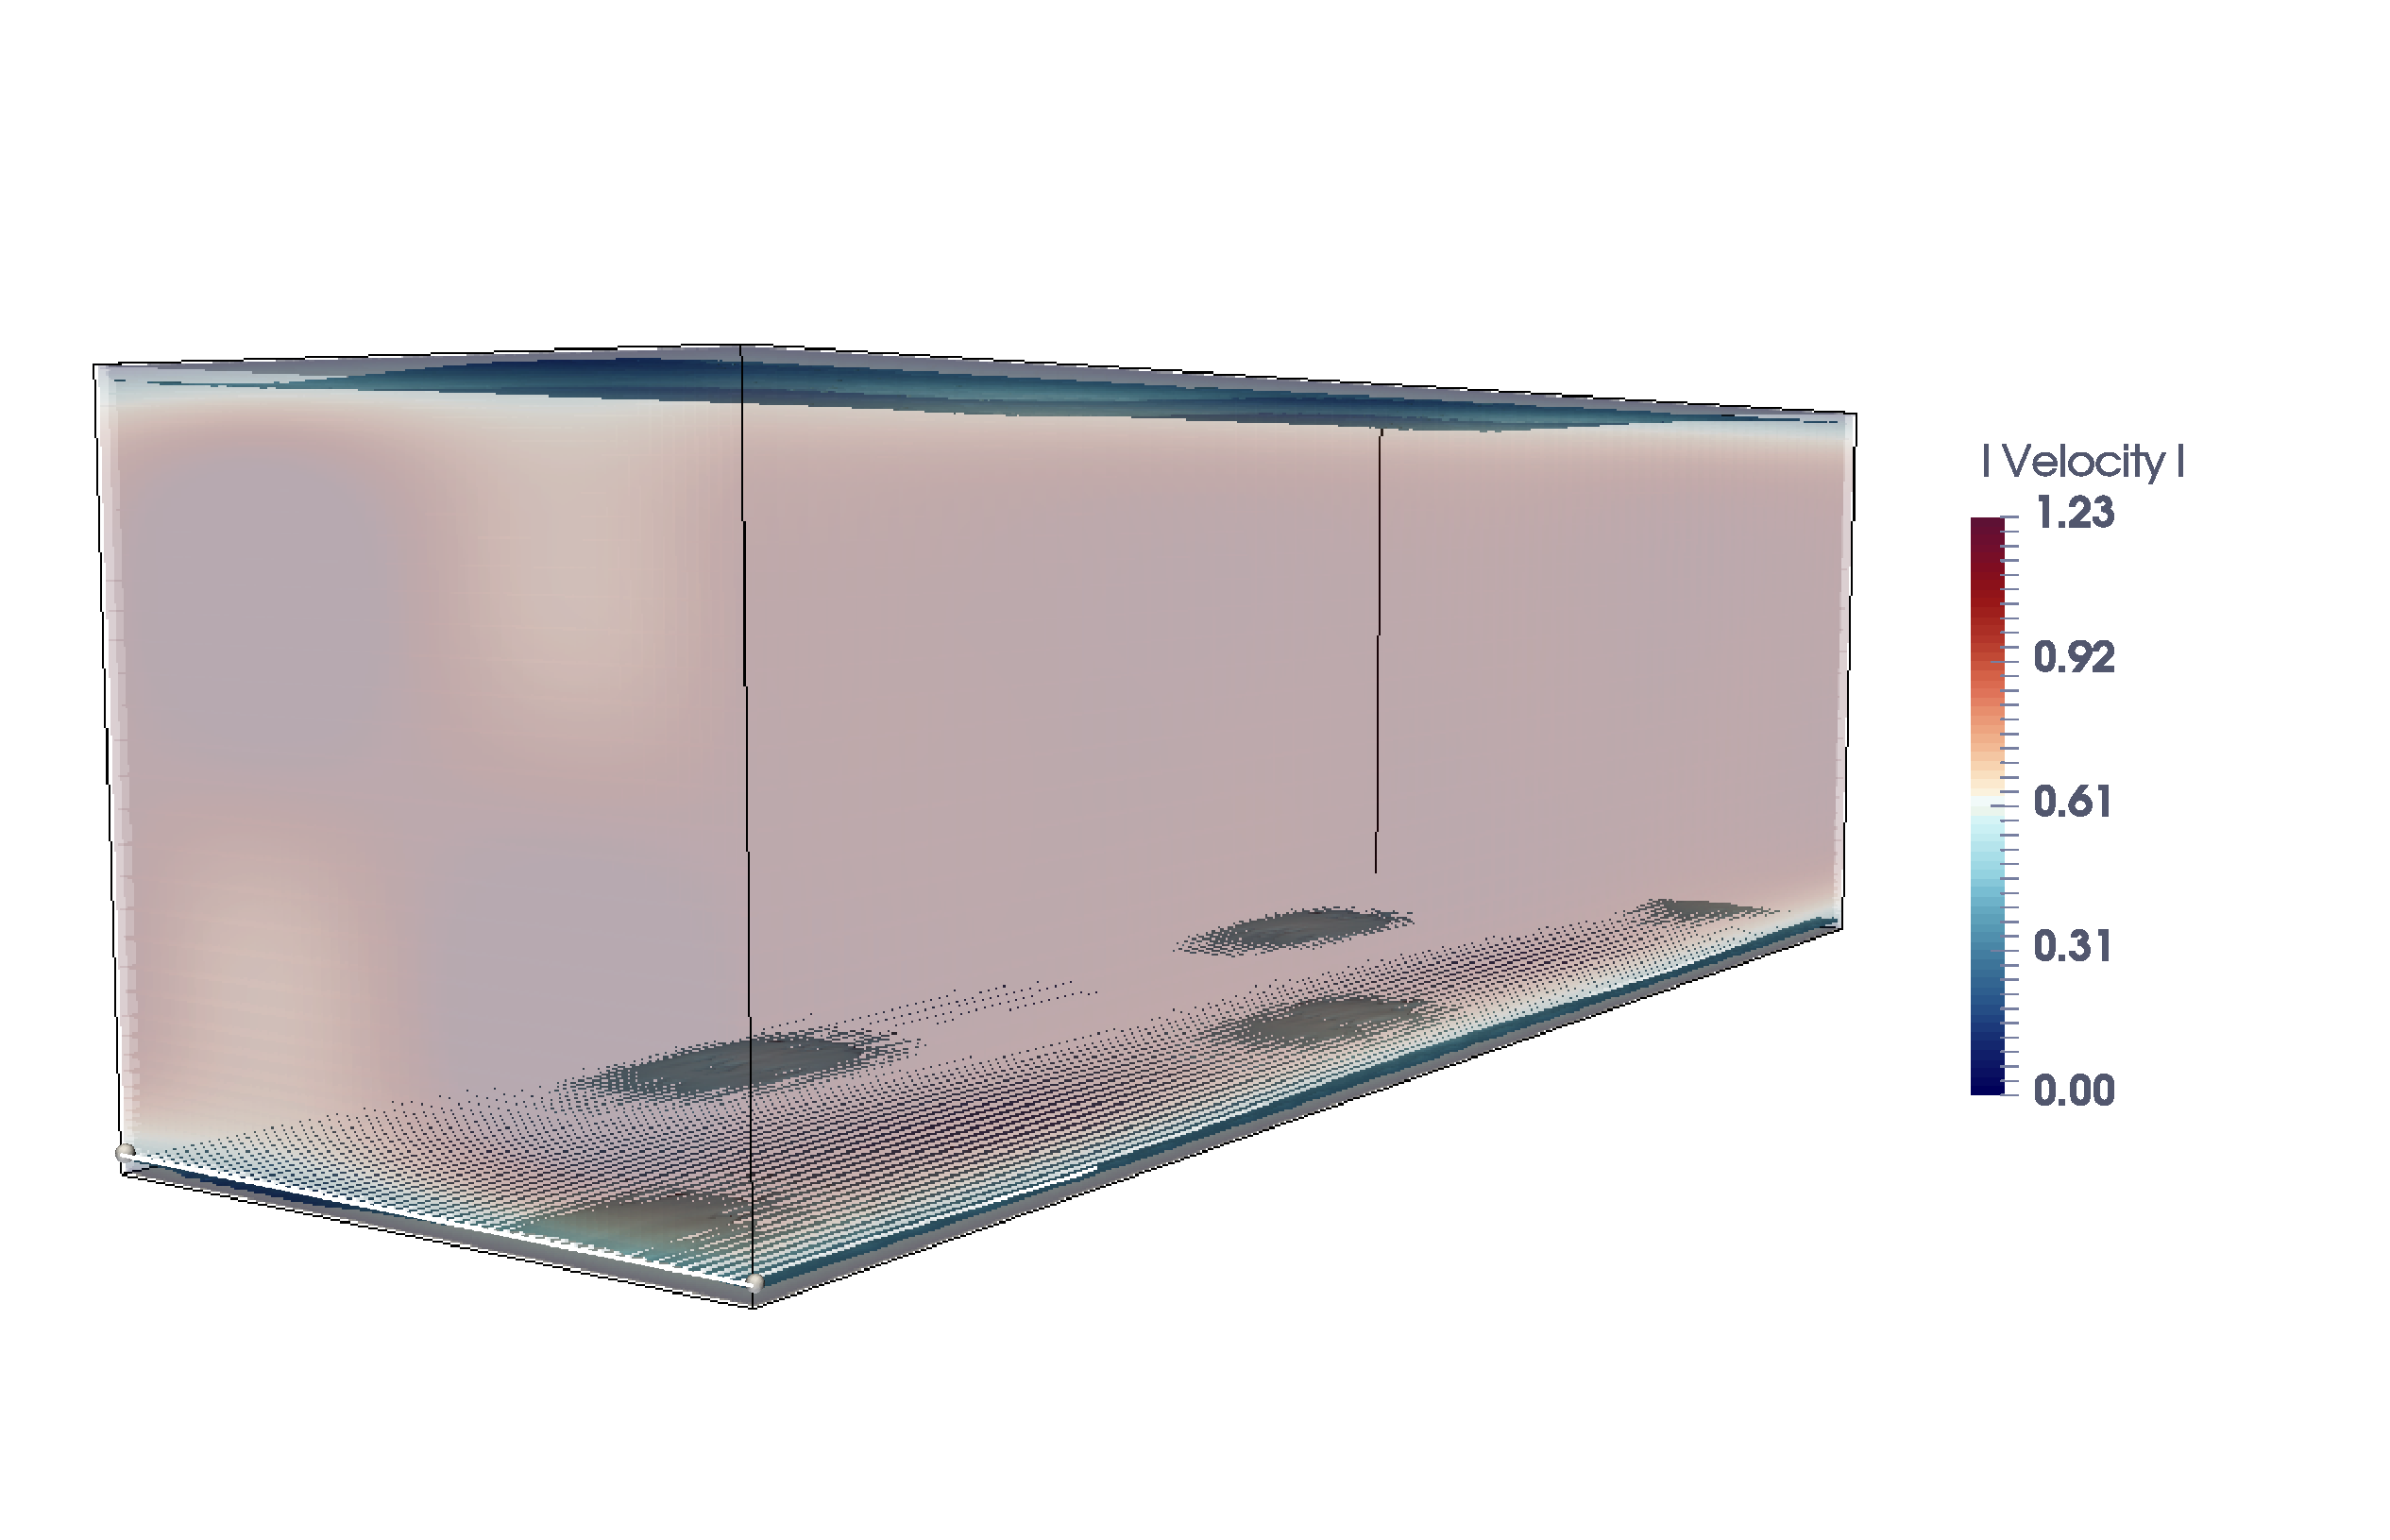
\includegraphics[width=0.49\textwidth,clip=true,trim=0.0cm 4.0cm 9.0cm 6.0cm]{Figures/Chapter5/TCF/divergence/ktauc/cha395_32el_0dot15}}
  \subfigure[$t=12.0$]{\label{fig-cha_c2_1.0_vel_12.0}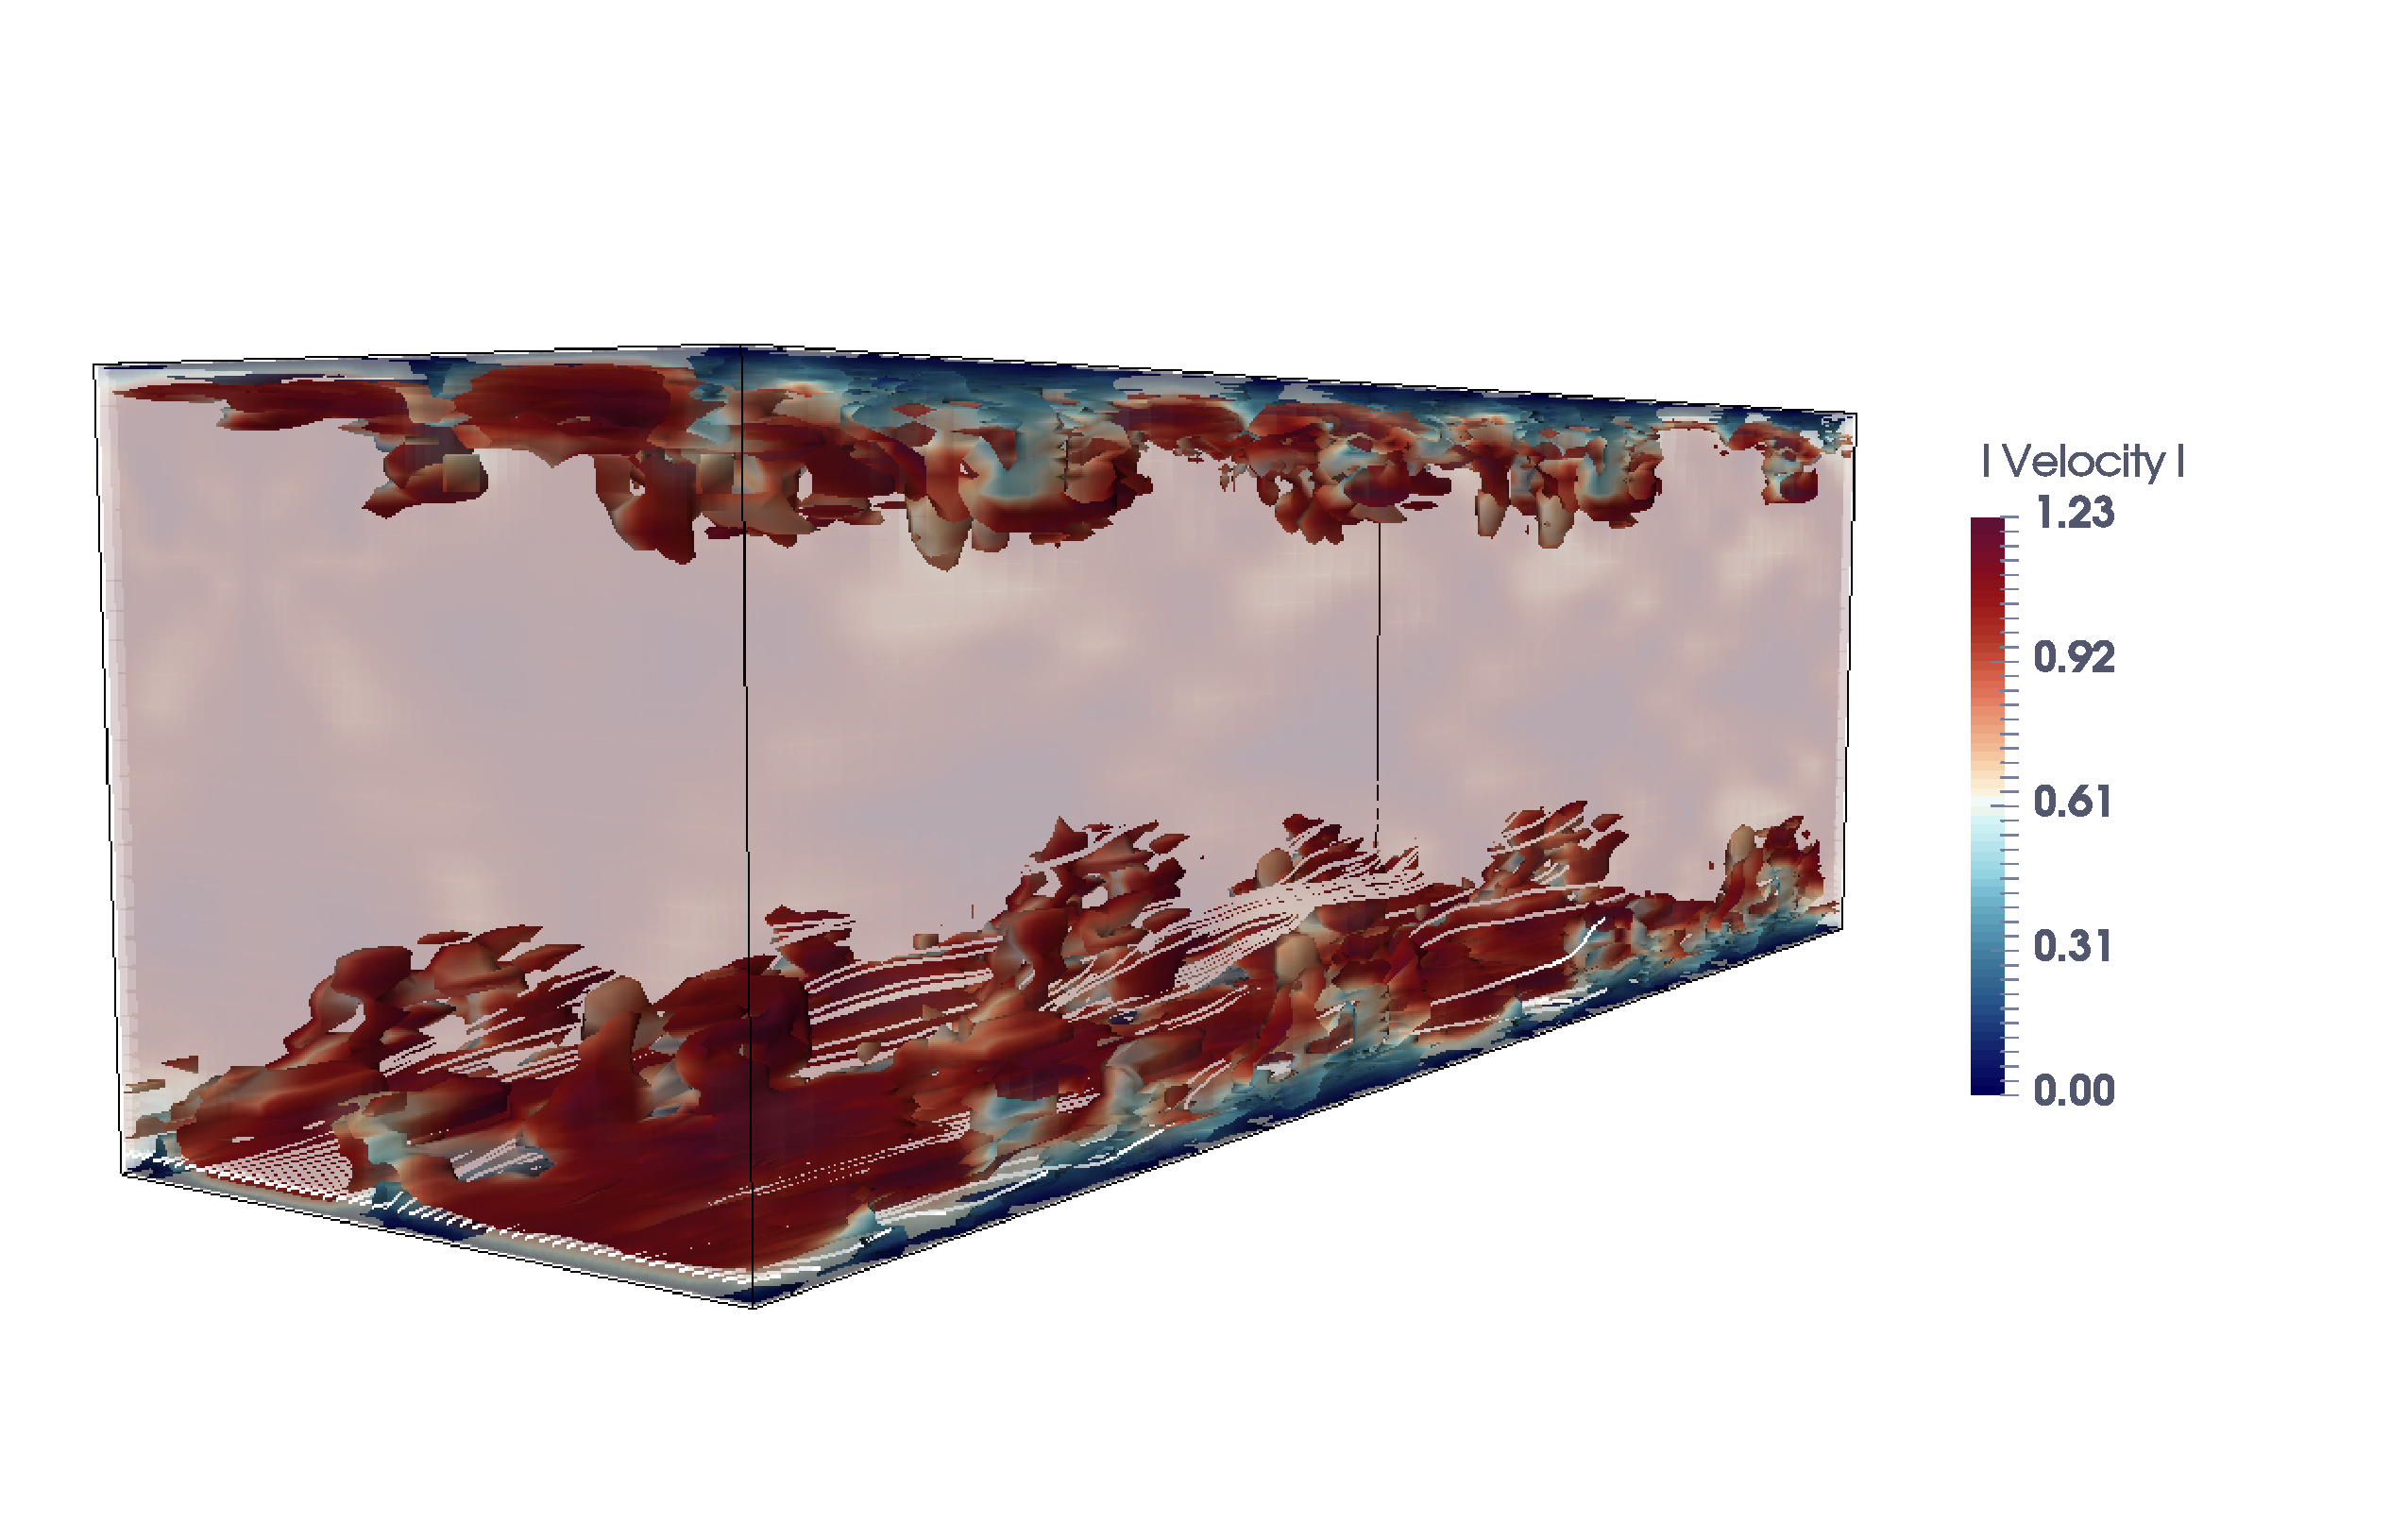
\includegraphics[width=0.49\textwidth,clip=true,trim=0.0cm 4.0cm 9.0cm 6.0cm]{Figures/Chapter5/TCF/divergence/ktauc/cha395_32el_12}}\\
  \subfigure[$t=70.0$]{\label{fig-cha_c2_1.0_vel_60.0}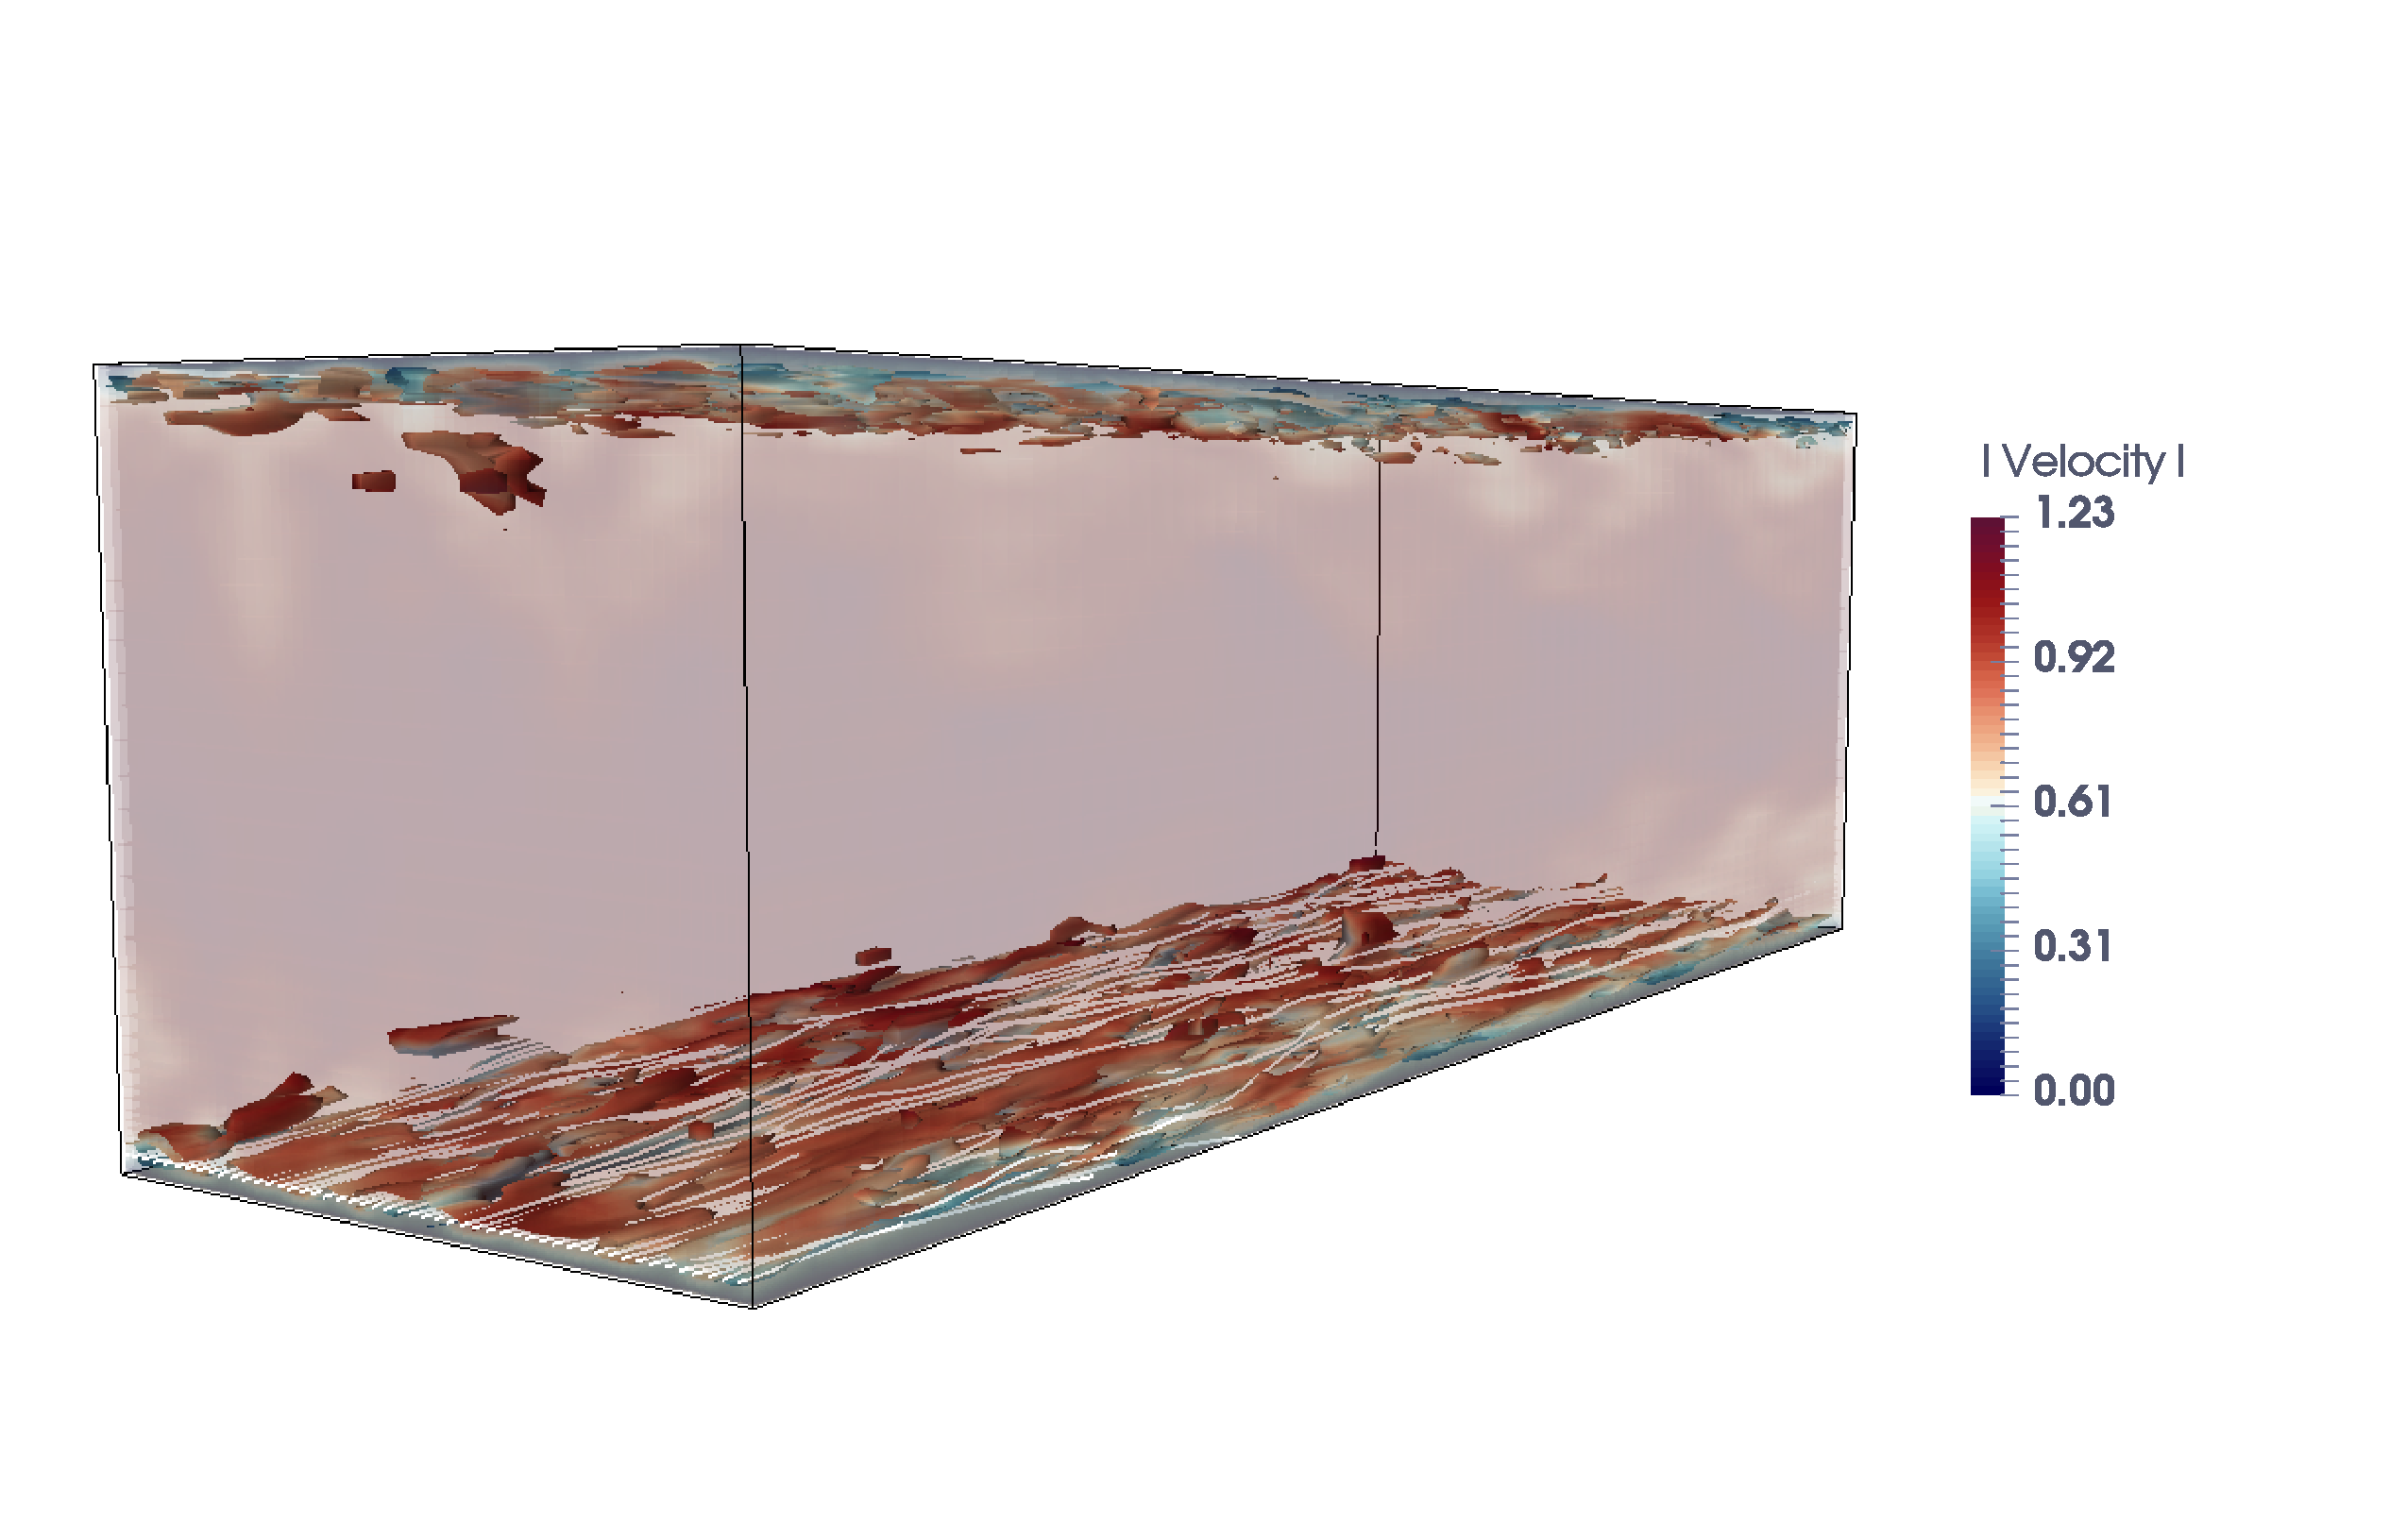
\includegraphics[width=0.49\textwidth,clip=true,trim=0.0cm 4.0cm 9.0cm 6.0cm]{Figures/Chapter5/TCF/divergence/ktauc/cha395_32el_70}}
  \subfigure{\label{fig-cha_c2_1.0_vel_60.0}\hspace{2.8cm}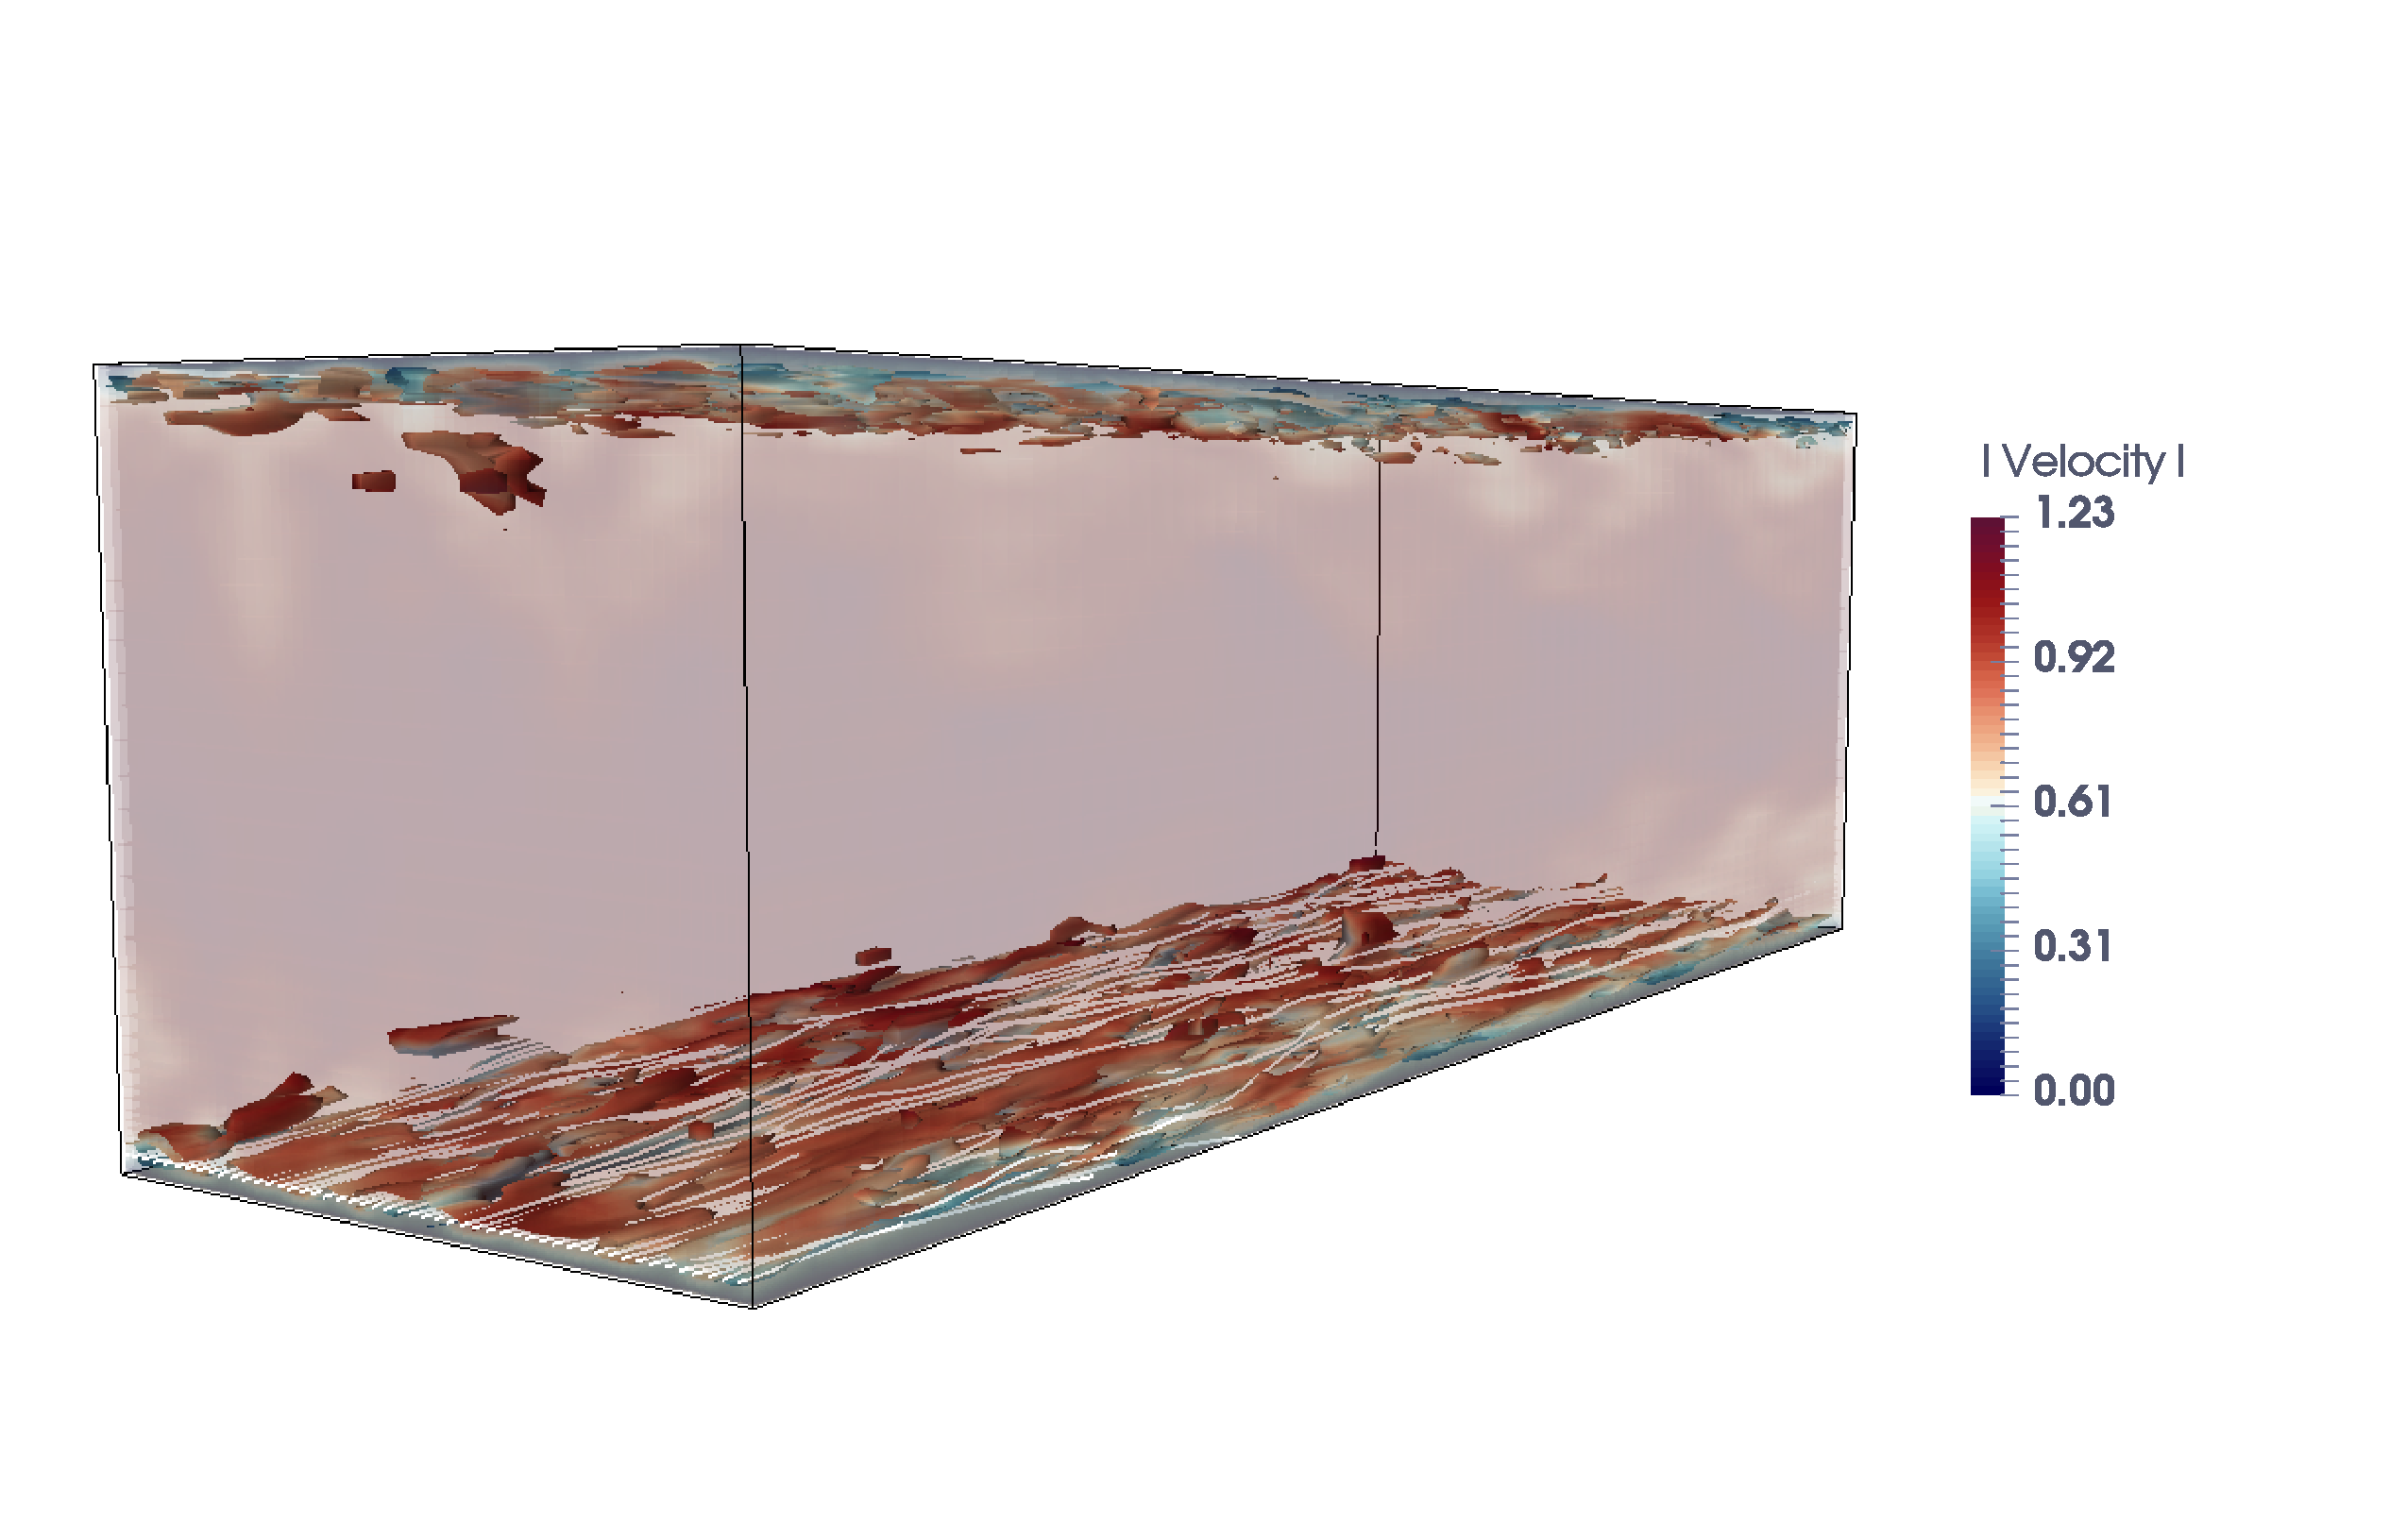
\includegraphics[width=0.1\textwidth,clip=true,trim=35.0cm 7.0cm 3.0cm 8.0cm]{Figures/Chapter5/TCF/divergence/ktauc/cha395_32el_70}\hspace{2.8cm}}
  \caption{Velocity module at different times with $c_1=12.0$, $c_2=1.0$ and $c_c=32.0$ using a $32^3$ $Q_2/Q_1$ elements mesh.}
  \label{fig-cha_c2_1.0_vel}
\end{figure}

When increasing $c_2$ we are decreasing the value of $\tau_m$, but increasing $\tau_c$. This means that in the energy dissipation equation \Eq{C5_ene_total}, the dissipation through the convective term $\|\tau_m^{1/2}(\u_h\cdot\nabla\u_h-\etaa_h)\|^2$ becomes less relevant in front of the $\|\tau_c^{1/2}\nabla\cdot\u_h\|^2$.

Now, knowing the influence of $c_2$, and with the aim to distinguish the effect of modifying $\tau_m$ or $\tau_c$, we keep this constant fixed with a value $c_2=8.0$ and we analyse the influence of $\tau_c$ on the solution, by changing $c_c$. In this situation, $\tau_m$ will remain constant for all cases and we will see the effect of the pressure subscale term. For this test, we solve the problem until $t=300$, where the energy evolution stabilizes for all $c_c$ choices.
\begin{figure}[h!]
  \centering
  \subfigure[Energy evolution]{\label{fig-cha_cc_ene}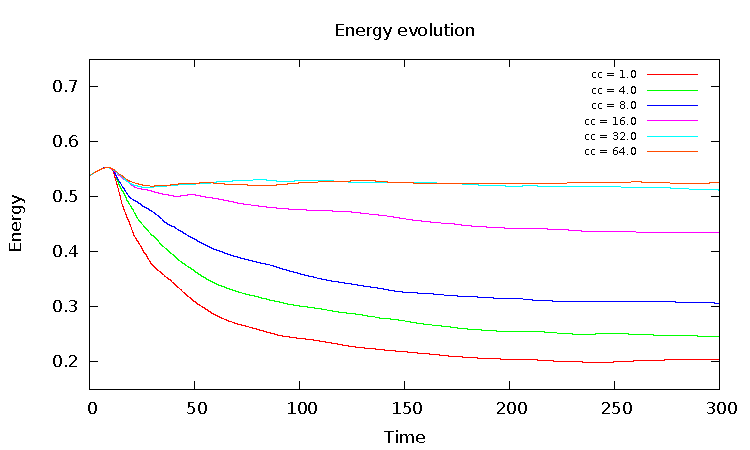
\includegraphics[width=0.49\textwidth]{Figures/Chapter5/TCF/divergence/ktauc/ene}}
  \subfigure[$\|\nabla\cdot\u_h\|$]{\label{fig-cha_cc_div}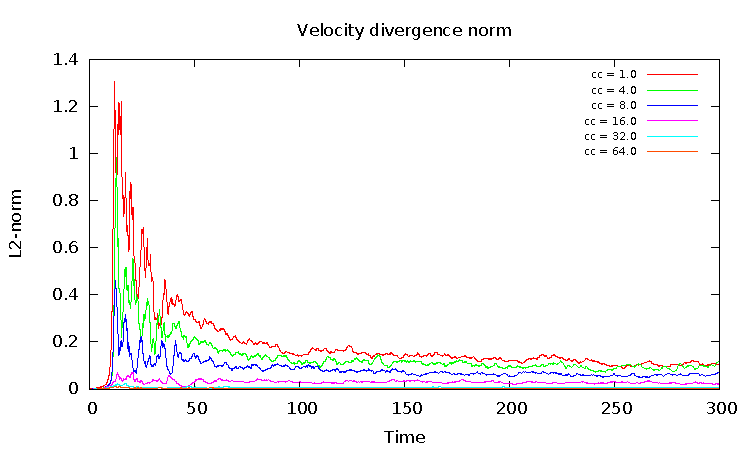
\includegraphics[width=0.49\textwidth]{Figures/Chapter5/TCF/divergence/ktauc/divel}}
  \caption{Energy evolution and velocity divergence norm for different values of $c_c$, keeping $c_1=12.0$ and $c_2=8.0$}
  \label{fig-cha_cc}
\end{figure}
In \Fig{cha_cc} we see that the energy evolution (\Fig{cha_cc_ene}) and the divergence norm evolution (\Fig{cha_cc_div}) follow the same pattern observed in \Fig{cha_c2}. In this case we see that the improvement on the mass conservation is more pronounced when increasing $c_c$ than when increasing $c_2$. We also see in \Fig{cha_cc_ene} that there is a certain threshold after which the result is improving very little. In this case, the results for $c_c=32.0$ and $c_c=64.0$ are almost the same.

We can compare our results with the MKM-DNS, contrasting the mean velocity and its fluctuations in \Fig{cha_cc_16}. To obtain these results we have solved the problem from $t=300$ to $t=330$ with a time step size of $\delta t=0.03$, collecting $1000$ samples to obtain the mean quantities. The mean quantities are computed integrating the desired quantity within each element and adding up all elemental results belonging to the same $y$-orthogonal plane. Thus, since we are using high-order elements, the number of points that will appear in the graphics will be smaller than the number of DOFs. This procedure was also followed in \cite{gamnitzer_time-dependent_2010} noting that the integral averaging procedure takes into account information from the secondary nodes that the widely used point-wise averaging does not contemplate.

\Fig{cha_cc_16_umean} depicts the mean stream-wise velocity normalized by the prescribed wall-shear velocity, $u_\tau$. In this picture we see the difference when changing $c_c$, where the dissipation of energy shown in \Fig{cha_cc_ene} becomes clear looking at the velocity magnitude. The increase of $\|\nabla\cdot\u_h\|$, and its consequent loss of mass conservation, results in a mean velocity profile much lower than the DNS. We see that for $c_c=32.0$ and $c_c=64.0$ the mean velocity profile is on top of the DNS result, even for the coarse mesh in which we are solving the problem. 
\begin{figure}[h!]
	\centering	
	\subfigure[Mean stream-wise velocity]{\label{fig-cha_cc_16_umean}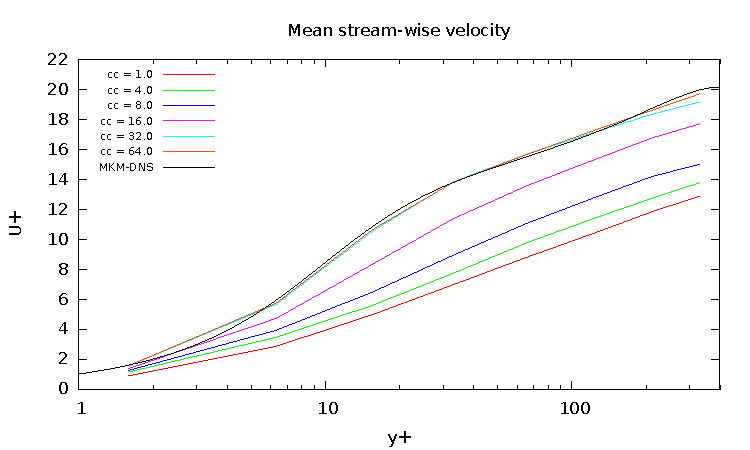
\includegraphics[width=0.49\textwidth]{Figures/Chapter5/TCF/divergence/ktauc/umean}}
	\subfigure[Rms stream-wise velocity fluctuation]{\label{fig-cha_cc_16_ufluc}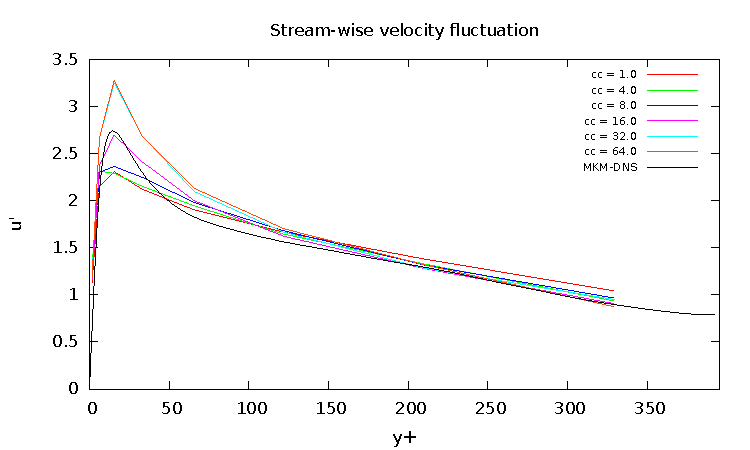
\includegraphics[width=0.49\textwidth]{Figures/Chapter5/TCF/divergence/ktauc/ufluc}}\\   
  	\subfigure[Rms wall-normal velocity fluctuation]{\label{fig-cha_cc_16_vfluc}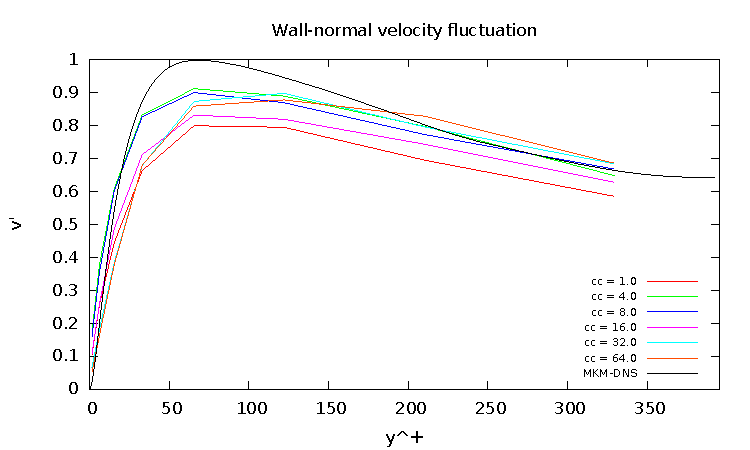
\includegraphics[width=0.49\textwidth]{Figures/Chapter5/TCF/divergence/ktauc/vfluc}}
  	\subfigure[Rms span-wise velocity fluctuation]{\label{fig-cha_cc_16_wfluc}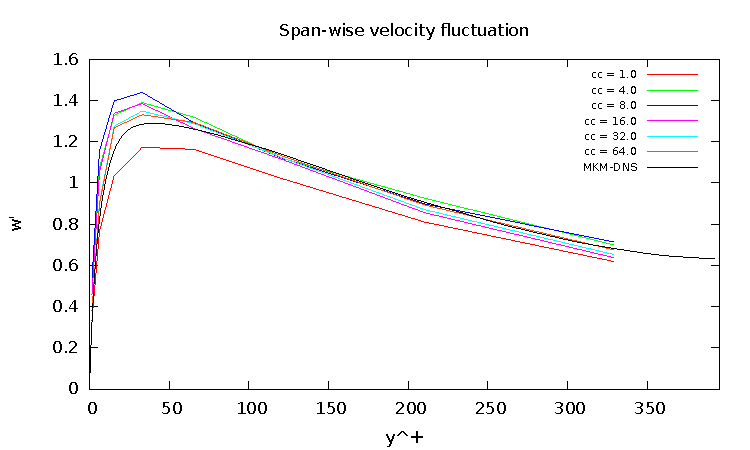
\includegraphics[width=0.49\textwidth]{Figures/Chapter5/TCF/divergence/ktauc/wfluc}}
	\caption{Mean stream-wise velocity and rms velocity fluctuations using a $16^3$ $Q_2/Q_1$ mesh for different choices of $c_c$.}
	\label{fig-cha_cc_16}
\end{figure}
Looking at the stream-wise velocity fluctuation (\Fig{cha_cc_16_ufluc}) we see that it increases as we increase $c_c$. This behaviour is justified by the fact that for low $c_c$ values we have less energy in the system, and then, the fluctuating magnitude is also lower. The wall-normal and span-wise velocity fluctuations also give the smallest fluctuation magnitude for the smallest $c_c$ value, but increasing $c_c$ the fluctuation grows until certain point and then it decreases, becoming closer to the DNS curve.

From \Fig{cha_cc_16} we clearly see that increasing $c_c$ the results improve, but this procedure may have some drawbacks. One of them is the ill-conditioning of the system of equations when $c_c\rightarrow\infty$. Table \ref{tab-cha_cc_16} summarizes the total accumulated solver iterations as well as the elapsed time needed to solve the problem for the different choices of $c_c$.
\begin{table}[h]
\caption{Solver iterations and elapsed time to solve the TCF problem from $t=300$ to $t=330$ for different $c_c$ values.}
\label{tab-cha_cc_16}
\centering
\begin{tabular}{cccc}
\toprule
$c_c$&Solver iterations&Elapsed time (s)&Increment in time ($\%$)\\
\midrule
\midrule
$1.0$&$397899$&$19238$&$0.0$\\
$4.0$&$402490$&$19674$&$2.27$\\
$8.0$&$422217$&$19987$&$3.89$\\
$16.0$&$466687$&$20803$&$8.13$\\
$32.0$&$539879$&$22794$&$18.48$\\
$64.0$&$626487$&$24817$&$29.00$\\
\bottomrule
\end{tabular}
\end{table}
As we see in Table \ref{tab-cha_cc_16}, to solve the TCF problem with $c_c=64.0$ is a $29.0\%$ more expensive than solving it with $c_c=1.0$. Thus, it is clear that at some point it could be preferable to refine the mesh rather than increase the $c_c$ value if we want more accurate results. 

Provided that in all results shown until now, the case $c_c=32.0$ gives almost the same solution as the $c_c=64.0$ case, hereinafter we will only consider the case in which the parametric constants are $c_1=12.0$, $c_2=8.0$ and $c_c=32.0$.

\subsubsection{Refinement for a given $c_c$}
Let us now explore what happens when the mesh is refined in the TCF test. Here we consider four different discretizations changing both the element size and the order of interpolation: $16^3$ $Q_2/Q_1$, $24^3$ $Q_2/Q_1$, $16^3$ $Q_3/Q_2$ and $32^3$ $Q_2/Q_1$. These discretizations have $32^3$, $48^3$, $48^3$ and $64^3$ velocity DOFs, respectively.

Looking at the energy evolution (\Fig{cha_refinement_ene}) and the velocity divergence $L_2$-norm (\Fig{cha_refinement_div}) depicted in \Fig{cha_refinement} we see that there are very little differences between the cases considered in this section. This means that given the appropriate parametric constants, the energy evolves in a similar way for all discretizations, with a similar evolution of the mass conservation. 
\begin{figure}[h!]
  \centering
  \subfigure[Energy evolution]{\label{fig-cha_refinement_ene}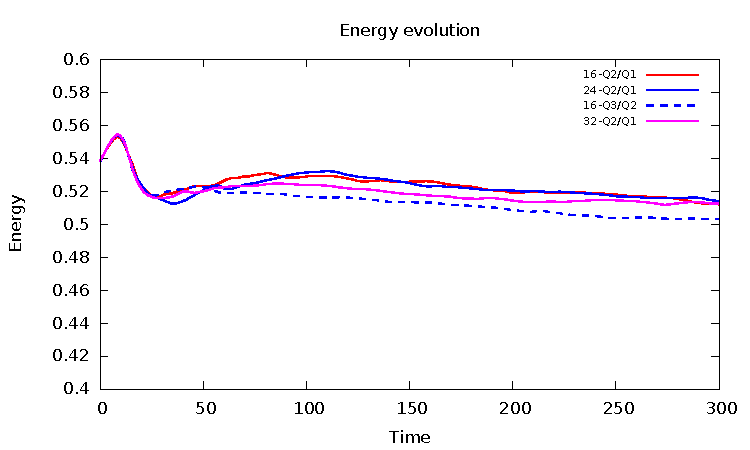
\includegraphics[width=0.49\textwidth]{Figures/Chapter5/TCF/refinement/ene}}
  \subfigure[$\|\nabla\cdot\u_h\|$]{\label{fig-cha_refinement_div}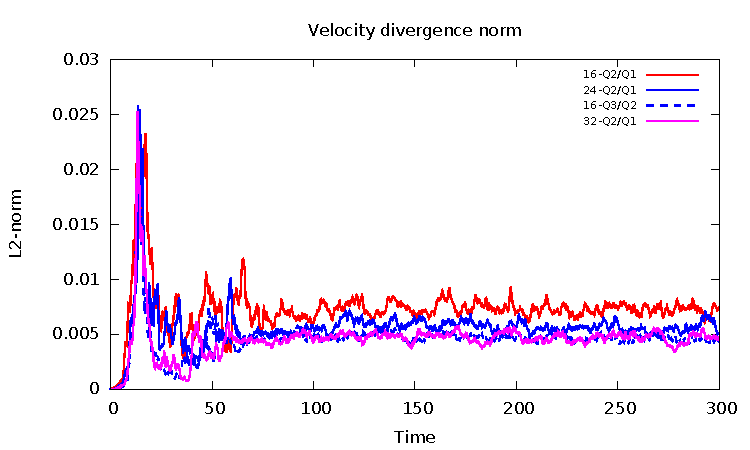
\includegraphics[width=0.49\textwidth]{Figures/Chapter5/TCF/refinement/divel}}
  \caption{Energy evolution and velocity divergence norm refining the mesh, keeping $c_1=12.0$, $c_2=8.0$ and $c_c=32.0$}
  \label{fig-cha_refinement}
\end{figure}

If we focus on the averaged turbulent quantities shown in \Fig{cha_refinement_vel}, we also see similar results between the different cases. In \Fig{cha_refinement_umean} the mean stream-wise velocity is plotted, and it is seen that all methods are almost on top of the DNS curve. The $16^3$ $Q_3/Q_2$ discretization gives  a mean velocity profile slightly lower than the other discretizations, which is also reflected on the energy evolution shown in \Fig{cha_refinement_ene}. If we look at the velocity fluctuations in span-wise, wall-normal, and span-wise directions depicted in \Fig{cha_refinement_ufluc}, \Fig{cha_refinement_vfluc} and \Fig{cha_refinement_wfluc}, respectively, the convergence to the DNS solution is clear.
\begin{figure}[h!]
	\centering	
	\subfigure[Mean stream-wise velocity]{\label{fig-cha_refinement_umean}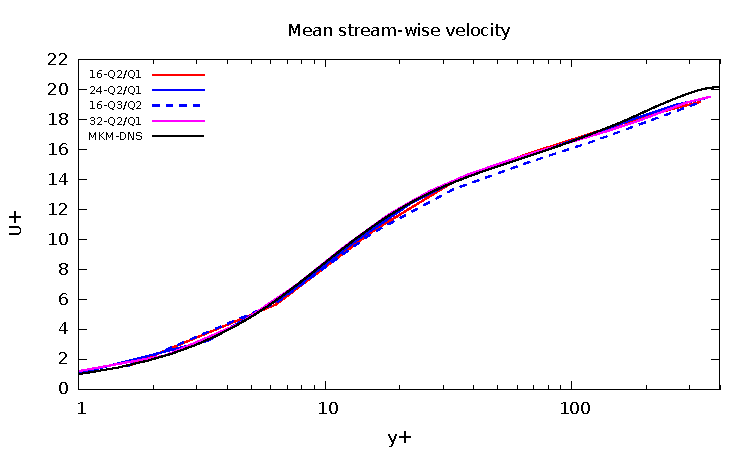
\includegraphics[width=0.49\textwidth]{Figures/Chapter5/TCF/refinement/umean}}
	\subfigure[Rms stream-wise velocity fluctuation]{\label{fig-cha_refinement_ufluc}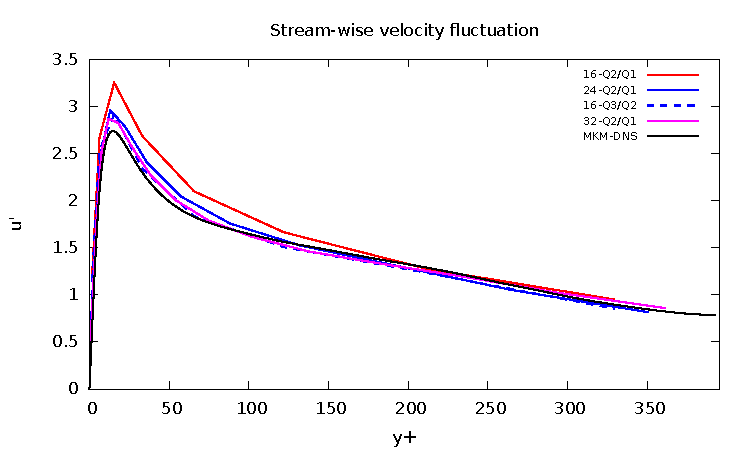
\includegraphics[width=0.49\textwidth]{Figures/Chapter5/TCF/refinement/ufluc}}\\   
  	\subfigure[Rms wall-normal velocity fluctuation]{\label{fig-cha_refinement_vfluc}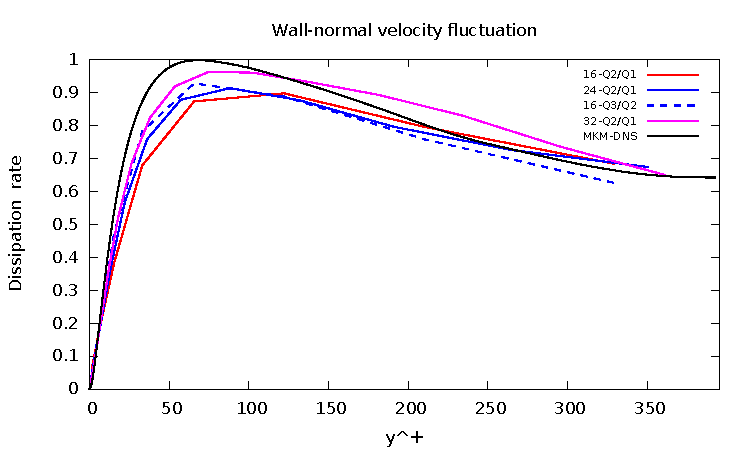
\includegraphics[width=0.49\textwidth]{Figures/Chapter5/TCF/refinement/vfluc}}
  	\subfigure[Rms span-wise velocity fluctuation]{\label{fig-cha_refinement_wfluc}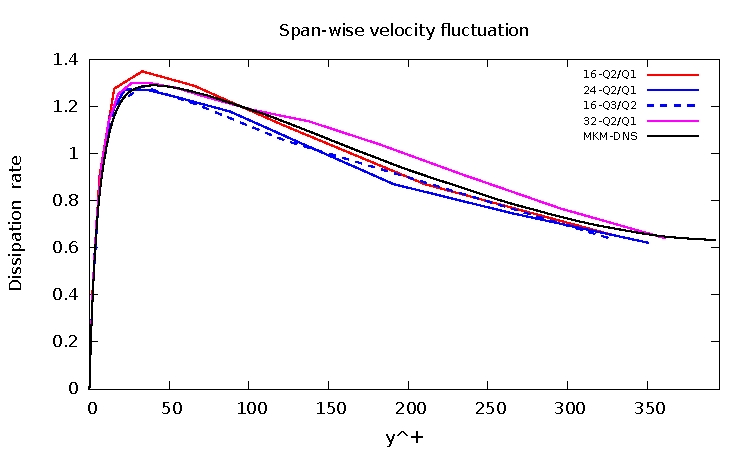
\includegraphics[width=0.49\textwidth]{Figures/Chapter5/TCF/refinement/wfluc}}
	\caption{Mean stream-wise velocity and rms velocity fluctuations for using different discretizations.}
	\label{fig-cha_refinement_vel}
\end{figure}

\section{Conclusions}
\label{sec-C5_conclusions}
In this chapter we have considered the numerical simulation of turbulent incompressible flows using the term-by-term OSS method for convection-stabilization applied to ISS elements. We have considered an implicit treatment of the projection. For the solution of the monolithic linear systems a  block preconditioning strategy that makes use of recursive block factorizations has been proposed. Among the three variants we proposed, namely diagonal, lower and upper triangular, the last two are much faster than the first one, as expected, the upper triangular being slightly faster for the problems considered. 

Using this strategy, the comparison of the three methods, ASGS, term-by-term OSS, and convection-only OSS with ISS elements reveals that the accuracy is similar for the same order of interpolation of the velocity, the OSS-ISS being slightly inferior in this respect. But on the other hand, when computational cost is analyzed the OSS-ISS is clearly the cheapest one so a finer discretization can be used. Another advantage of the OSS-ISS method is that it does not change the nature in time of the problem, i.e., the discrete system is an index-2 differential-algebraic equation. Thus, it allow us, e.g., to use Segregated Runge-Kutta (SRK) time integration schemes that cannot be applied to the ASGS or OSS methods. This issue will be discussed in further works, but we can say that SRK schemes are well suited to perform high-order time integration as well as the use of an adaptive time-stepping technique. This method was firstly introduced and tested for laminar incompressible flows in \cite{colomes_segregated_2015} and will be discussed in forthcoming chapters.

Finally, we have also analyzed the influence of the grad-div stabilization on the results when ISS discretizations are considered. It has been clearly shown that this term affects the solution. Increasing the value of $c_c$ results in a better mass conservation and better results but this saturates at some point from which little improvements are achieved while we have a high increase on the computational cost. Moreover, this effect is smaller when the mesh is refined and also when higher order interpolations are used.